
\subsection{Two Dimensional Plot Types}
{
\tikzset{external/figure name/.add={}{twodim_}}%
\PGFPlots\ supports several two-dimensional line plots like piecewise linear line plots, piecewise constant plots, smoothed plots, bar plots and comb plots. Most of them use the \PGF\ plot handler library directly, see \cite[section 18.8]{tikz}.

Plot types are part of the plot style, so they are set with options. Most of the basic 2d plot types are part of \Tikz, see \cite[section 18.8]{tikz}, and are probably known to users of \Tikz. They are documented here as well.


\subsubsection{Linear Plots}
\begin{plottype}{sharp plot}
Linear (`sharp') plots are the default. Point coordinates are simply connected by straight lines. 
\begin{codeexample}[]
\begin{tikzpicture}
\begin{axis}
	\addplot+[sharp plot] coordinates 
		{(0,0) (1,2) (2,3)};
\end{axis}
\end{tikzpicture}
\end{codeexample}

The `|+|' here means to use the normal plot cycle list and append `|sharp plot|' to its option list.
\end{plottype}

\subsubsection{Smooth Plots}
\begin{plottype}{smooth}
Smooth plots interpolate smoothly between successive points.
\begin{codeexample}[]
\begin{tikzpicture}
\begin{axis}
	\addplot+[smooth] coordinates 
		{(0,0) (1,2) (2,3)};
\end{axis}
\end{tikzpicture}
\end{codeexample}
\end{plottype}

\subsubsection{Constant Plots}
Constant plots draw lines parallel to the $x$-axis to connect coordinates. The discontinuous edges may be drawn or not, and marks may be placed on left or right ends.

\begin{plottype}{const plot}
Connects all points with horizontal and vertical lines. Marks are placed left-handed on horizontal line segments, causing the plot to be right-sided continuous at all data points.

\begin{codeexample}[]
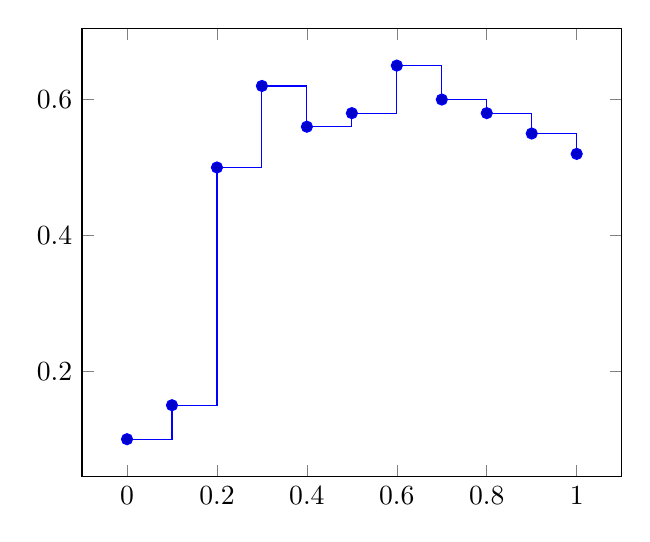
\begin{tikzpicture}
\begin{axis}
\addplot+[const plot]
coordinates
{(0,0.1)    (0.1,0.15)  (0.2,0.5)   (0.3,0.62)
 (0.4,0.56) (0.5,0.58)  (0.6,0.65)  (0.7,0.6)
 (0.8,0.58) (0.9,0.55)  (1,0.52)};
\end{axis}
\end{tikzpicture}
\end{codeexample}


\begin{codeexample}[]
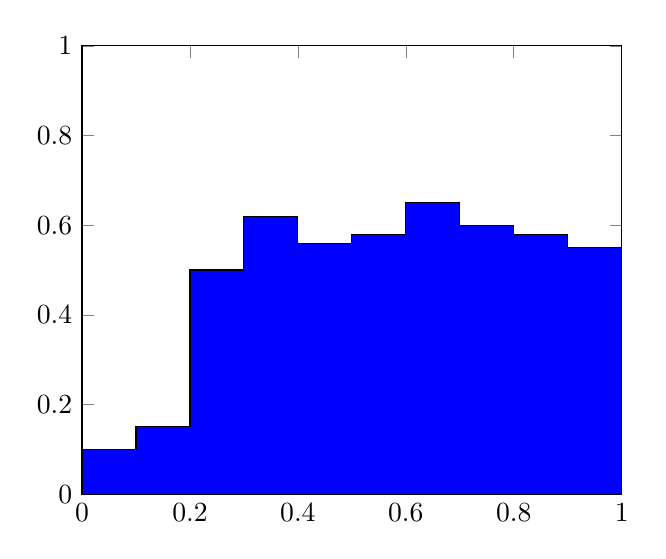
\begin{tikzpicture}
\begin{axis}[ymin=0,ymax=1,enlargelimits=false]
\addplot
	[const plot,fill=blue,draw=black] 
coordinates
{(0,0.1)    (0.1,0.15)  (0.2,0.5)   (0.3,0.62)
 (0.4,0.56) (0.5,0.58)  (0.6,0.65)  (0.7,0.6)
 (0.8,0.58) (0.9,0.55)  (1,0.52)} 
	\closedcycle;
\end{axis}
\end{tikzpicture}
\end{codeexample}
\end{plottype}

\begin{plottype}{const plot mark left}
An alias for `|const plot|'.
\end{plottype}

\begin{plottype}{const plot mark right}
 A variant which places marks on the right of each line segment, causing plots to be left-sided continuous at the given coordinates.
\begin{codeexample}[]
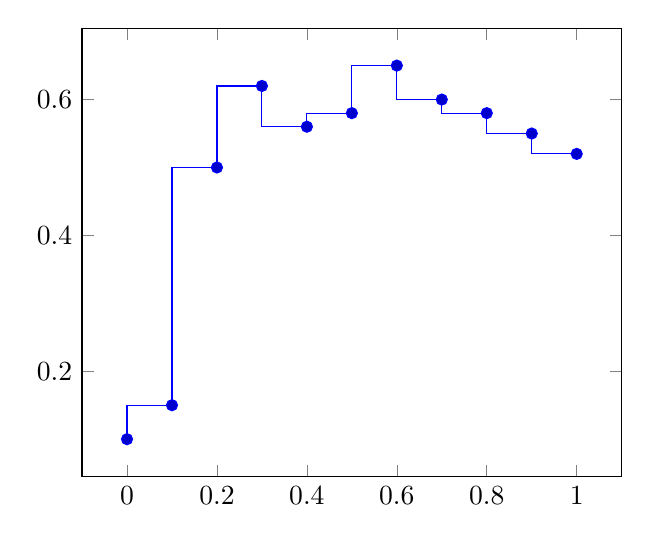
\begin{tikzpicture}
\begin{axis}
\addplot+[const plot mark right]
coordinates
{(0,0.1)    (0.1,0.15)  (0.2,0.5)   (0.3,0.62)
 (0.4,0.56) (0.5,0.58)  (0.6,0.65)  (0.7,0.6)
 (0.8,0.58) (0.9,0.55)  (1,0.52)};
\end{axis}
\end{tikzpicture}
\end{codeexample}
\end{plottype}

\begin{plottype}{const plot mark mid}
 A variant which places marks in the middle of each line segment, causing plots to be symmetric around its data points.
\begin{codeexample}[]
\begin{tikzpicture}
\begin{axis}
\addplot+[const plot mark mid]
coordinates
{(0,0.1)    (0.1,0.15)  (0.2,0.5)   (0.3,0.62)
 (0.4,0.56) (0.5,0.58)  (0.6,0.65)  (0.7,0.6)
 (0.8,0.58) (0.9,0.55)  (1,0.52)};
\end{axis}
\end{tikzpicture}
\end{codeexample}
	Note that ``symmetric'' is only true for constant mesh width: if the $x$--distances between adjacent data points differ, |const plot mark mid| will produce vertical lines in the middle between each pair of consecutive points.
\end{plottype}

\begin{plottype}{jump mark left}
A variant of `|const plot mark left|' which does not draw vertical lines.
\begin{codeexample}[]
\begin{tikzpicture}
\begin{axis}[samples=8]
\addplot+[jump mark left,domain=-5:0] 
	{4*x^2 - 5};

\addplot+[jump mark right,domain=-5:0] 
	{0.7*x^3 + 50};
\end{axis}
\end{tikzpicture}
\end{codeexample}
\end{plottype}

\begin{plottype}{jump mark right}
A variant of `|const plot mark right|' which does not draw vertical lines.
\end{plottype}

\begin{plottype}{jump mark mid}
 A variant of `|const plot mark mid|' which does not draw vertical lines.
\begin{codeexample}[]
\begin{tikzpicture}
\begin{axis}
\addplot+[jump mark mid]
coordinates
{(0,0.1)    (0.1,0.15)  (0.2,0.5)   (0.3,0.62)
 (0.4,0.56) (0.5,0.58)  (0.6,0.65)  (0.7,0.6)
 (0.8,0.58) (0.9,0.55)  (1,0.52)};
\end{axis}
\end{tikzpicture}
\end{codeexample}
\end{plottype}

\subsubsection{Bar Plots}
Bar plots place horizontal or vertical bars at coordinates. Multiple bar plots in one axis can be stacked on top of each other or aligned next to each other.

\begin{plottype}{xbar}
	Places horizontal bars between the $(y=0)$ line and each coordinate.

	This option is used on a per-plot basis and configures only the visualization of coordinates. The figure-wide style |/pgfplots/xbar| also sets reasonable options for ticks, legends and multiple plots.
\begin{codeexample}[]
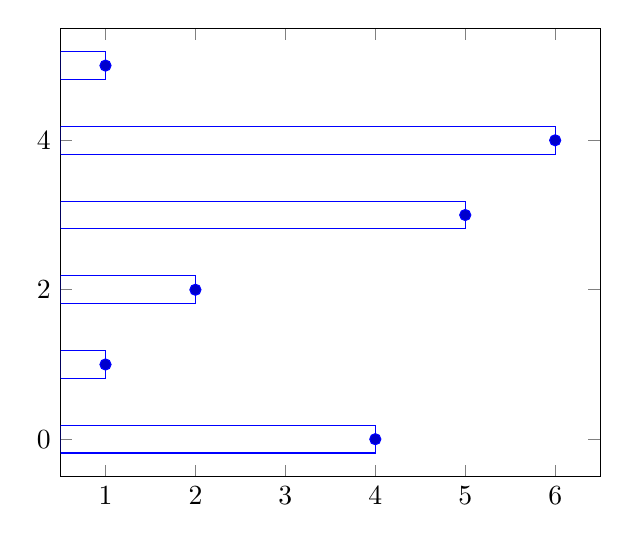
\begin{tikzpicture}
\begin{axis}
\addplot+[xbar] coordinates 
	{(4,0) (1,1) (2,2) 
	 (5,3) (6,4) (1,5)};
\end{axis}
\end{tikzpicture}
\end{codeexample}
	Bars are centered at plot coordinates with width |bar width|. Using bar plots usually means more than just a different way of how to connect coordinates, for example to draw ticks outside of the axis, change the legend's appearance or introduce shifts if multiple |\addplot| commands appear.

	There is a preconfigured style for |xbar| which is installed automatically if you provide |xbar| as argument to the axis environment which provides this functionality.
% \usetikzlibrary{patterns}
\begin{codeexample}[]
\begin{tikzpicture}
\begin{axis}[xbar,enlargelimits=0.15]
\addplot
[draw=blue,pattern=horizontal lines light blue] 
coordinates
	{(10,5) (15,10) (5,15) (24,20) (30,25)};

\addplot
[draw=black,pattern=horizontal lines dark blue] 
coordinates 
	{(3,5) (5,10) (15,15) (20,20) (35,25)};
\end{axis}
\end{tikzpicture}
\end{codeexample}
Here |xbar| yields |/pgfplots/xbar| because it is an argument to the axis, not to a single plot.

	For bar plots, it is quite common to provide textual coordinates or even descriptive nodes near the bars.
	This can be implemented using the keys |symbolic y coords| and |nodes near coords|, respectively:
\begin{codeexample}[]
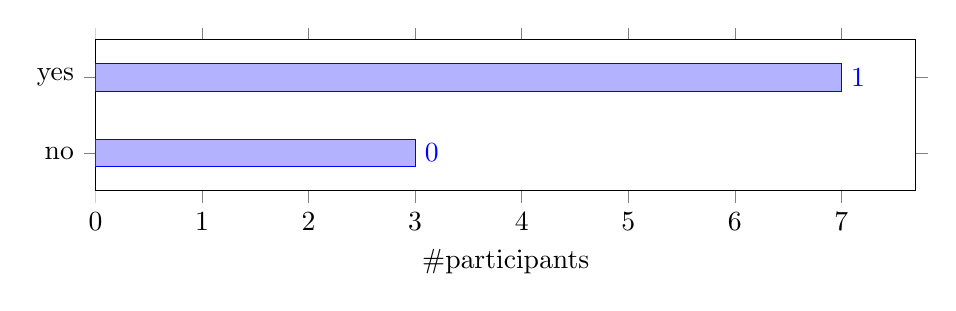
\begin{tikzpicture}
  \begin{axis}[
    xbar, xmin=0,
    width=12cm, height=3.5cm, enlarge y limits=0.5,
    xlabel={\#participants},
    symbolic y coords={no,yes},
    ytick=data,
    nodes near coords, nodes near coords align={horizontal},
    ]
    \addplot coordinates {(3,no) (7,yes)};
  \end{axis}
\end{tikzpicture}
\end{codeexample}
	The |symbolic y coords| defines a dictionary of accepted coordinates which are then expected in $y$ coordinates and the |nodes near coords| key displays values as extra nodes (see their reference documentations for details). The example employs |enlarge y limits| in order to get some more free space since the default spacing is not always appropriate for bar plots.

	Note that it might be quite important to include |xmin=0| explicitly as in the example above. Without it, the lower bound will be used:
\begin{codeexample}[]
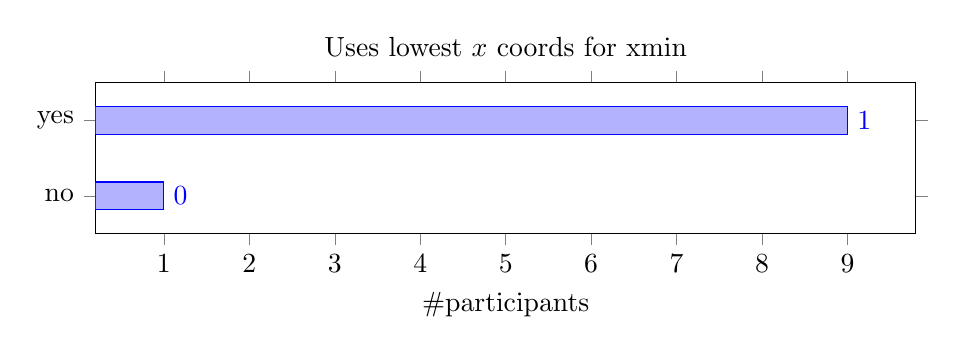
\begin{tikzpicture}
  \begin{axis}[
  	title=Uses lowest $x$ coords for xmin,
    xbar,
    width=12cm, height=3.5cm, enlarge y limits=0.5,
    xlabel={\#participants},
    symbolic y coords={no,yes},
    ytick=data,
    nodes near coords, nodes near coords align={horizontal},
    ]
    \addplot coordinates {(1,no) (9,yes)};
  \end{axis}
\end{tikzpicture}
\end{codeexample}

	Besides line, fill, and colorstyles, bars can be configured with |bar width| and |bar shift|, see below.
\end{plottype}

\begin{stylekey}{/pgfplots/xbar=\marg{shift for multiple plots} (default 2pt)}
	This style sets |/tikz/xbar| \emph{and} some commonly used options concerning horizontal bars for the complete axis. This is automatically done if you provide |xbar| as argument to an axis argument, see above.

The |xbar| style defines shifts if multiple plots are placed into one axis. It draws bars adjacent to each other, separated by \meta{shift for multiple plots}. Furthermore, it sets the style |bar cycle list| and sets tick and legend appearance options.

The style is defined as follows.
\begin{codeexample}[code only]
\pgfplotsset{
	/pgfplots/xbar/.style={
		/tikz/xbar,
		bar cycle list,
		tick align=outside,
		xbar legend,
		/pgf/bar shift={%
			% total width = n*w + (n-1)*skip
			% i.e. subtract half for centering
			-0.5*(\numplotsofactualtype*\pgfplotbarwidth + (\numplotsofactualtype-1)*#1)  + 
			% the '0.5*w' is for centering
			(.5+\plotnumofactualtype)*\pgfplotbarwidth + \plotnumofactualtype*#1%
		},
	},
}
\end{codeexample}
The formula for |bar shift| assigns shifts dependent on the total number of plots and the current plot's number. It is designed to fill a total width of $n \cdot $|bar width|$ + (n-1) \cdot $\meta{shift for multiple plots}. The $0.5$ compensates for centering.
\end{stylekey}

\begin{plottype}{ybar}
	Like |xbar|, this option generates bar plots. It draws vertical bars between the ($x=0$) line and each input coordinate.
\begin{codeexample}[]
\begin{tikzpicture}
\begin{axis}
\addplot+[ybar] plot coordinates
	{(0,3) (1,2) (2,4) (3,1) (4,2)};
\end{axis}
\end{tikzpicture}
\end{codeexample}
	The example above simply changes how input coordinates shall be visualized. As mentioned for |xbar|, one usually needs modified legends and shifts for multiple bars in the same axis.

	There is a predefined style which installs these customizations when provided to the axis environment:
\begin{codeexample}[]
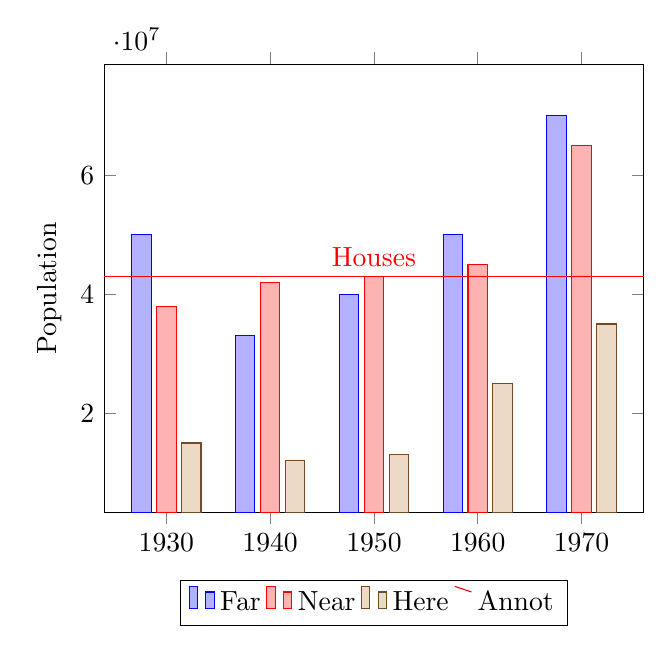
\begin{tikzpicture}
\begin{axis}[
	x tick label style={
		/pgf/number format/1000 sep=},
	ylabel=Population,
	enlargelimits=0.15,
	legend style={at={(0.5,-0.15)},
		anchor=north,legend columns=-1},
	ybar,
	bar width=7pt,
]
\addplot 
	coordinates {(1930,50e6) (1940,33e6)
		 (1950,40e6) (1960,50e6) (1970,70e6)};

\addplot 
	coordinates {(1930,38e6) (1940,42e6) 
		(1950,43e6) (1960,45e6) (1970,65e6)};

\addplot 
	coordinates {(1930,15e6) (1940,12e6) 
		(1950,13e6) (1960,25e6) (1970,35e6)};

\addplot[red,sharp plot,update limits=false] 
	coordinates {(1910,4.3e7) (1990,4.3e7)} 
	node[above] at (axis cs:1950,4.3e7) {Houses};

\legend{Far,Near,Here,Annot}
\end{axis}
\end{tikzpicture}
\end{codeexample}
Here, |ybar| yields |/pgfplots/ybar| because it is an argument to the axis, not to a single plot. The style affects the first three |\addplot| commands. Note that it shifts them horizontally around the plot coordinates. The fourth |\addplot| command is some kind of annotation which doesn't |update limits|.

	The |ybar| style can be combined with |symbolic x coords| in a similar way as described for |xbar|:
\begin{codeexample}[]
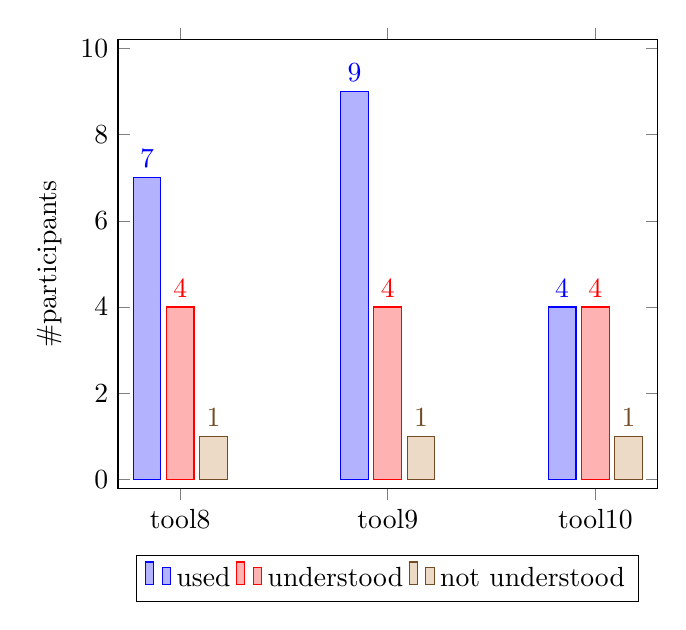
\begin{tikzpicture}
\begin{axis}[
    ybar,
    enlargelimits=0.15,
    legend style={at={(0.5,-0.15)},
      anchor=north,legend columns=-1},
    ylabel={\#participants},
    symbolic x coords={tool8,tool9,tool10},
    xtick=data,
    nodes near coords,
    nodes near coords align={vertical},
    ]
\addplot coordinates {(tool8,7) (tool9,9) (tool10,4)};
\addplot coordinates {(tool8,4) (tool9,4) (tool10,4)};
\addplot coordinates {(tool8,1) (tool9,1) (tool10,1)};
\legend{used,understood,not understood}
\end{axis}
\end{tikzpicture}
\end{codeexample}

	As for |xbar|, the bar width and shift can be configured with |bar width| and |bar shift|. However, the bar shift is better provided as argument to |/pgfplots/ybar| since this style will overwrite the bar shift. Thus, prefer |/pgfplots/ybar=4pt| to set the bar shift.

	Sometimes it is useful to write the $y$ values directly near the bars. This can be realized using the |nodes near coords| method:
\begin{codeexample}[]
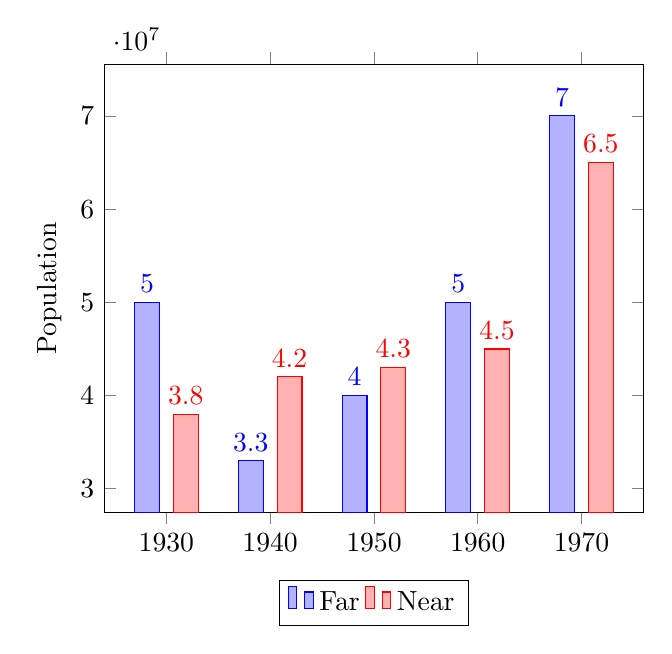
\begin{tikzpicture}
\begin{axis}[
	x tick label style={
		/pgf/number format/1000 sep=},
	ylabel=Population,
	enlargelimits=0.15,
	legend style={at={(0.5,-0.15)},
		anchor=north,legend columns=-1},
	ybar=5pt,% configures `bar shift'
	bar width=9pt,
	nodes near coords,
	point meta=y *10^-7 % the displayed number
]
\addplot 
	coordinates {(1930,50e6) (1940,33e6)
		 (1950,40e6) (1960,50e6) (1970,70e6)};

\addplot 
	coordinates {(1930,38e6) (1940,42e6) 
		(1950,43e6) (1960,45e6) (1970,65e6)};

\legend{Far,Near}
\end{axis}
\end{tikzpicture}
\end{codeexample}

	Any support style changes are possible, of course. A useful example for bar plots might be to use rotated tick labels:
\begin{codeexample}[]
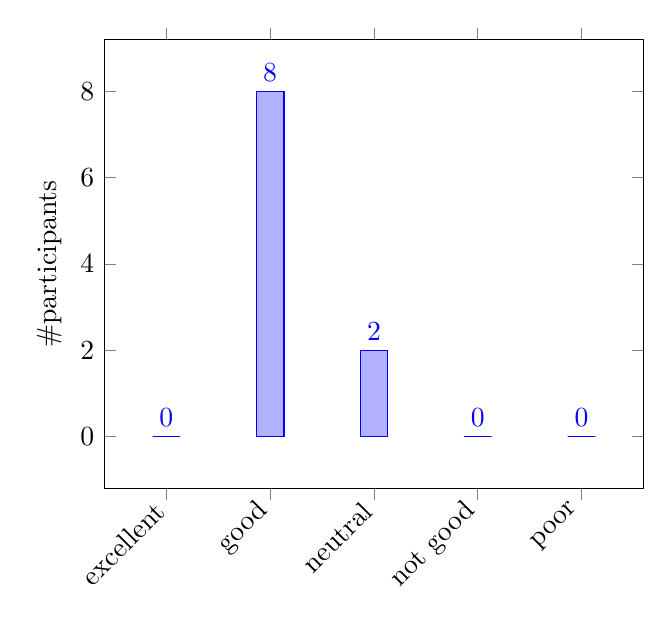
\begin{tikzpicture}
  \begin{axis}[
    ybar,
    enlargelimits=0.15,
    legend style={at={(0.5,-0.2)},
      anchor=north,legend columns=-1},
    ylabel={\#participants},
    symbolic x coords={excellent,good,neutral,%
		not good,poor},
    xtick=data,
    nodes near coords, 
	nodes near coords align={vertical},
    x tick label style={rotate=45,anchor=east},
    ]
    \addplot coordinates {(excellent,0) (good,8) 
		(neutral,2) (not good,0) (poor,0)};
  \end{axis}
\end{tikzpicture}
\end{codeexample}
\end{plottype}

\begin{stylekey}{/pgfplots/ybar=\marg{shift for multiple plots} (default 2pt)}
	As |/pgfplots/xbar|, this style sets the |/tikz/ybar| option to draw vertical bars, but it also provides commonly used options for vertical bars.

	If you supply |ybar| to an axis environment, |/pgfplots/ybar| will be chosen instead of |/tikz/ybar|.

	It changes the legend, draws ticks outside of the axis lines and draws multiple |\addplot| arguments adjacent to each other; block--centered at the $x$ coordinate and separated by \meta{shift for multiple plots}. It will also install the |bar shift| for |every node near coord|. Furthermore, it installs the style |bar cycle list|. It is defined similarly to |/pgfplots/xbar|.
\end{stylekey}

\begin{pgfplotskey}{bar cycle list}
	A style which installs cycle lists for multiple bar plots.
\begin{codeexample}[code only]
\pgfplotsset{
	/pgfplots/bar cycle list/.style={/pgfplots/cycle list={%
		{blue,fill=blue!30!white,mark=none},%
		{red,fill=red!30!white,mark=none},%
		{brown!60!black,fill=brown!30!white,mark=none},%
		{black,fill=gray,mark=none},%
		}
	},
}
\end{codeexample}
	
\end{pgfplotskey}

\begin{key}{/pgf/bar width=\marg{dimension or unit} (initially 10pt)}
	Configures the width used by |xbar| and |ybar|. It is accepted to provide mathematical expressions.

	As of \PGFPlots\ 1.7, it is allows to provide an \emph{unit} as |bar width|. In this case, the |bar width| will be interpreted as axis unit:
\begin{codeexample}[]
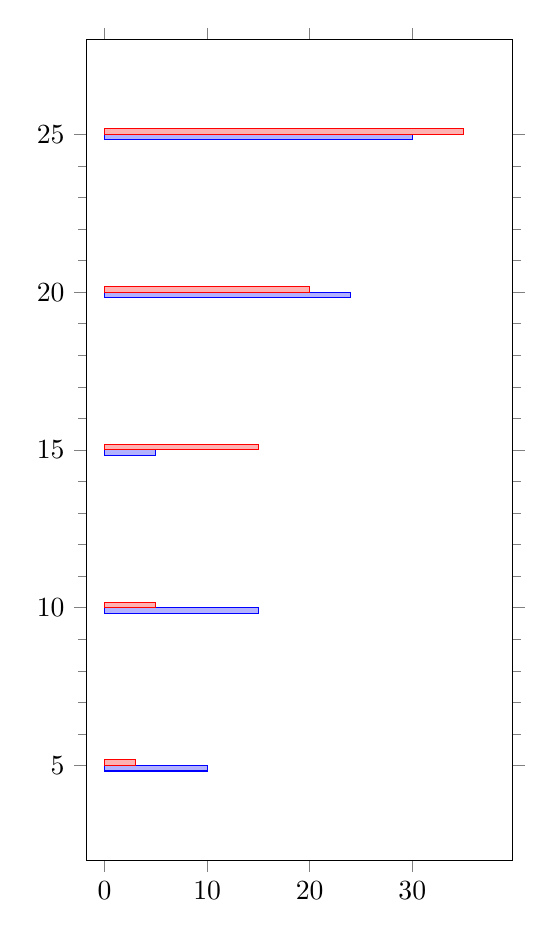
\begin{tikzpicture}
\begin{axis}[
	xbar=0pt,% space of 0pt between adjacent bars
	bar width=2,
	width=7cm,
	height=12cm,
	minor y tick num=4,
	ytick=data,
	enlargelimits=0.15]
\addplot
coordinates
    {(10,5) (15,10) (5,15) (24,20) (30,25)};
\addplot
coordinates
    {(3,5) (5,10) (15,15) (20,20) (35,25)};
\end{axis}
\end{tikzpicture}
\end{codeexample}
	In order to interprete arguments as units, you have to write |\pgfplotsset{compat=1.7}| (or newer) into your preamble. Older versions will implicitly append the |pt| suffix if the argument is no dimension.

	\begin{command}{\pgfplotbarwidth}
		A mathematical expression which results in the fully computed value of |bar width| (i.e.\ it includes any unit computations). 
	\end{command}

	Note that you may need to |enlargelimits| in order to see the complete bar -- \PGFPlots\ will not automatically update the axis limits to respect |bar width|.
\end{key}

\begin{key}{/pgf/bar shift=\marg{dimension or unit} (initially 0pt)}
	Configures a shift for |xbar| and |ybar|. Use |bar shift| together with |bar width| to draw multiple bar plots into the same axis. It is accepted to provide mathematical expressions.

	As of \PGFPlots\ 1.7, it is allows to provide an \emph{unit} as |bar shift|. In this case, the |bar shift| will be interpreted as axis unit.
	\begin{command}{\pgfplotbarshift}
		A mathematical expression which results in the fully computed value of |bar shift| (i.e.\ it includes any unit computations). 
	\end{command}
	Note that you may need to |enlargelimits| in order to see the complete bar -- \PGFPlots\ will not automatically update the axis limits to respect |bar shift|.
\end{key}


\begin{plottype}{ybar interval}
	This plot type produces vertical bars with width (and shift) relatively to intervals of coordinates.

	There is one conceptional difference when working with intervals: an interval is defined by \emph{two} coordinates. Since |ybar| has one value for each interval, the $i$th bar is defined by
	\begin{enumerate}
		\item the $y$ value of the $i$th coordinates,
		\item the $x$ value of the $i$th coordinate as left interval boundary,
		\item the $x$ value of the $(i+1)$th coordinate as right interval boundary.
	\end{enumerate}
	Consequently, there is \emph{one coordinate too much}: the last coordinate will \emph{only} be used to determine the interval width; its $y$ value doesn't influence the bar appearance.

	It is installed on a per-plot basis and configures \emph{only} the visualization of coordinates. See the style |/pgfplots/ybar interval| which configures the appearance of the complete figure.
\begin{codeexample}[]
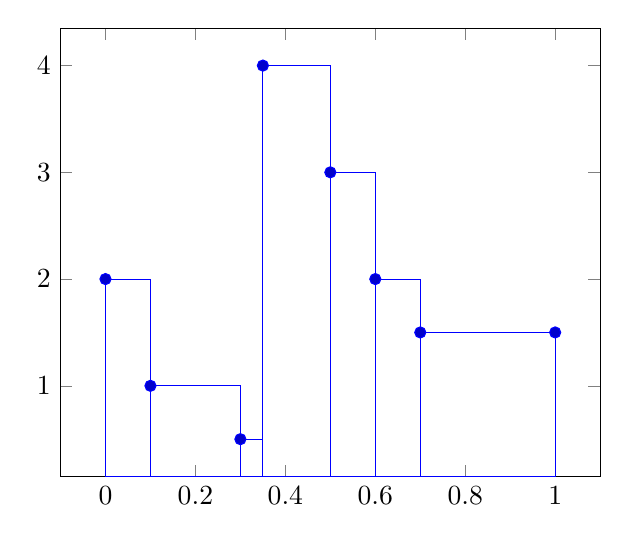
\begin{tikzpicture}
\begin{axis}
\addplot+[ybar interval] plot coordinates
	{(0,2) (0.1,1) (0.3,0.5) (0.35,4) (0.5,3)
	 (0.6,2) (0.7,1.5) (1,1.5)};
\end{axis}
\end{tikzpicture}
\end{codeexample}

\begin{codeexample}[]
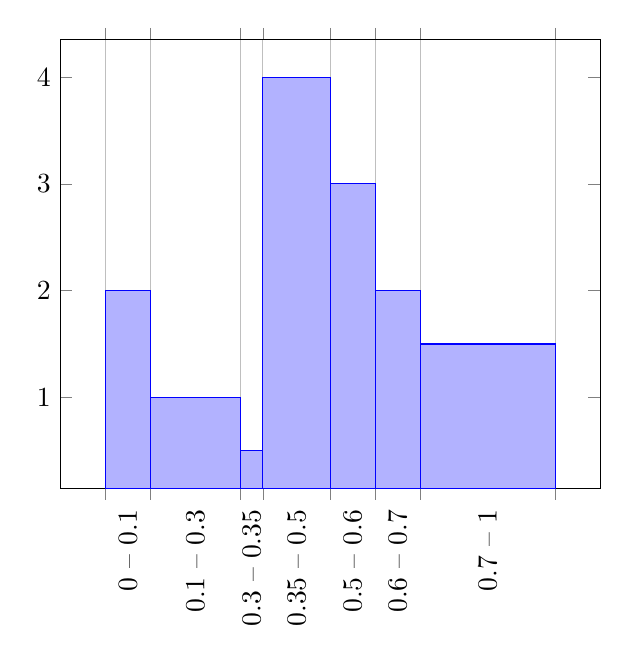
\begin{tikzpicture}
\begin{axis}[ybar interval,
	xtick=data,
	xticklabel interval boundaries,
	x tick label style=
		{rotate=90,anchor=east}
	]
\addplot coordinates
	{(0,2) (0.1,1) (0.3,0.5) (0.35,4) (0.5,3)
	 (0.6,2) (0.7,1.5) (1,1.5)};
\end{axis}
\end{tikzpicture}
\end{codeexample}

\begin{codeexample}[]
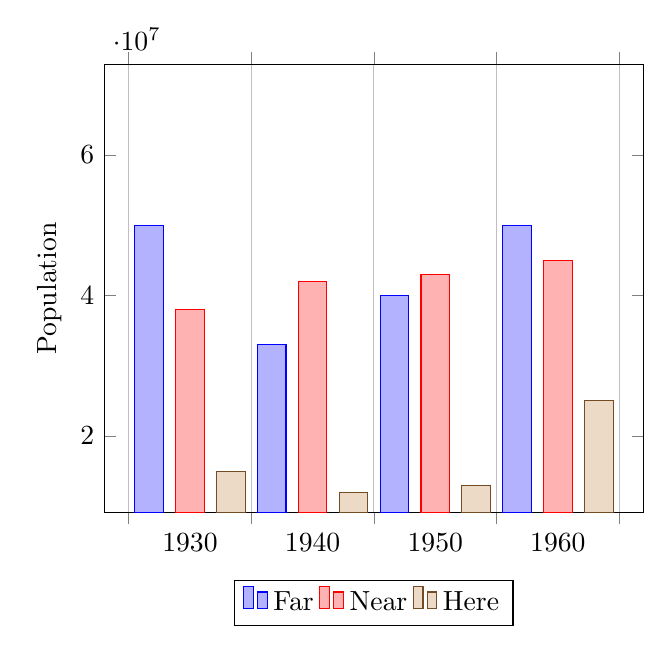
\begin{tikzpicture}
\begin{axis}[
	x tick label style={
		/pgf/number format/1000 sep=},
	ylabel=Population,
	enlargelimits=0.05,
	legend style={at={(0.5,-0.15)},
		anchor=north,legend columns=-1},
	ybar interval=0.7,
]
\addplot 
	coordinates {(1930,50e6) (1940,33e6)
		 (1950,40e6) (1960,50e6) (1970,70e6)};

\addplot 
	coordinates {(1930,38e6) (1940,42e6) 
		(1950,43e6) (1960,45e6) (1970,65e6)};

\addplot 
	coordinates {(1930,15e6) (1940,12e6) 
		(1950,13e6) (1960,25e6) (1970,35e6)};
\legend{Far,Near,Here}
\end{axis}
\end{tikzpicture}
\end{codeexample}
\end{plottype}

\begin{stylekey}{/pgfplots/ybar interval=\marg{relative width} (default 1)}
	A style which is intended to install options for |ybar interval| for a complete figure. This includes tick and legend appearance, management of multiple bar plots in one figure and a more adequate |cycle list| using the style |bar cycle list|.
\end{stylekey}

\begin{plottype}{xbar interval}
	As |ybar interval|, just for horizontal bars. 
\begin{codeexample}[]
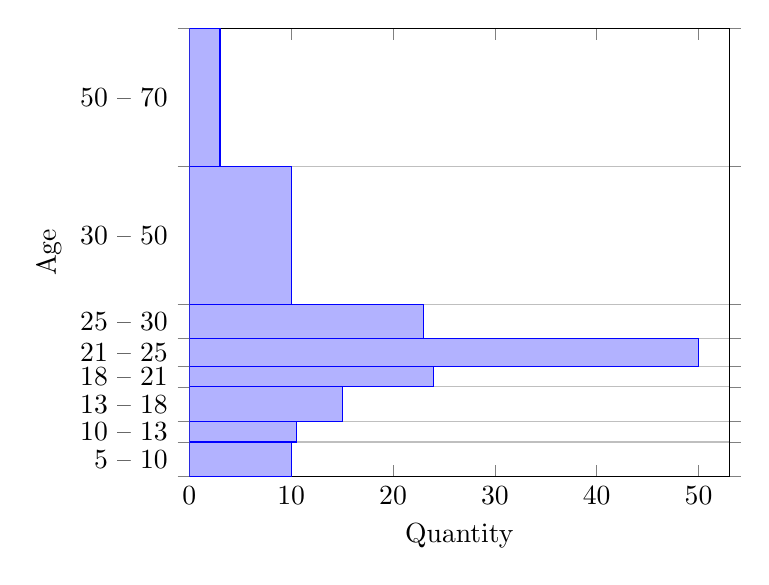
\begin{tikzpicture}
\begin{axis}[
	xmin=0,xmax=53,
	ylabel=Age,
	xlabel=Quantity,
	enlargelimits=false,
	ytick=data,
	yticklabel interval boundaries,
	xbar interval,
]
\addplot
	coordinates {(10,5) (10.5,10) (15,13) 
		(24,18) (50,21) (23,25) (10,30) 
		(3,50) (3,70)};
\end{axis}
\end{tikzpicture}
\end{codeexample}
\end{plottype}

\begin{stylekey}{/pgfplots/xbar interval=\marg{relative width} (default 1)}
	A style which is intended to install options for |xbar interval| for a complete figure, see the style |/pgfplots/ybar interval| for details.
\end{stylekey}

\begin{pgfplotsxykey}{\x ticklabel interval boundaries}
	These are style keys which set |x tick label as interval| (see page~\pageref{key:pgfplots:ticklabelasinterval} for details) and configure the tick appearance to be \meta{start} -- \meta{end} for each tick interval.
\end{pgfplotsxykey}

\subsubsection{Histograms}
\begin{plottype}[/pgfplots]{hist=\textcolor{black}{\normalfont\marg{options with {\normalfont\texttt{hist/}} prefix}}}
	A histogram plot takes one-dimensional input data and counts the occurrence of values: it determines the data range $[\underline m,\overline m]$ and subdivides it into $N$ equally sized bins with $(N+1)$ end--points. Then, it counts the number of points falling into each bin. More precisely, it computes the $N+1$ points $\underline m =: x_0 < x_1 < \dotsb < x_N := \overline m$ using $x_i := \underline m + i \cdot (\overline m - \underline m)/N$. Then, it creates the $N+1$ coordinates $(x_i, y_i)$, $i=0,\dotsc,N-1$ by means of
	\[
  y_i := 
  \begin{cases}
  \text{bincount}\bigl([x_i,x_{i+1})\bigr)\Bigr) & i<N\\
  y_{N-1} & i = N,
\end{cases}
	\]
	i.e.\ the value of the last coordinate is replicated.
	This set of $(N+1)$ interval boundaries is then visualized by an |ybar interval| plot handler.
\begin{codeexample}[]
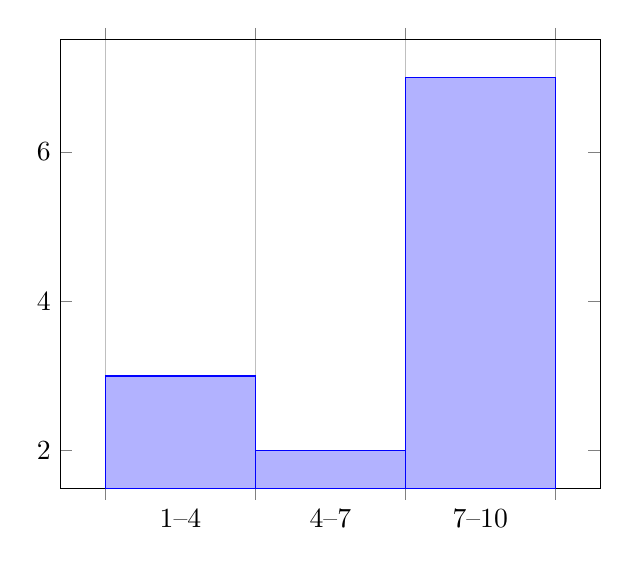
\begin{tikzpicture}
\begin{axis}[
  ybar interval,
  xticklabel=
\pgfmathprintnumber\tick--\pgfmathprintnumber\nexttick
]
	\addplot+[hist={bins=3}]
		table[row sep=\\,y index=0] {
		data\\
		1\\ 2\\ 1\\ 5\\ 4\\ 10\\ 
		7\\ 10\\ 9\\ 8\\ 9\\ 9\\ 
	};
\end{axis}
\end{tikzpicture}
\end{codeexample}
	We see that |hist={bins=3}| takes a table with one column as input. The data values fall into the range $[1,10]$ which is partitioned into~$3$ intervals (of equal lengths). Finally, the number of points falling into each of the three bins is plotted. The |xticklabel| key shows the range (note that it works only in conjunction with |x tick label as interval| which has been enabled by |ybar interval| before). We see that there are $3$ elements in the range $[1,4)$, $2$~elements in the range $[4,7)$ and finally $7$ elements in the range $[7,10]$. 
	
	The bins are half--open intervals, i.e.\ the end--point does not belong to the bin. Only the last bin contains its right end point.
\pgfplotsexpensiveexample
\begin{codeexample}[]
\begin{tikzpicture}
\begin{axis}[
  ybar interval,
  xtick=,% reset from ybar interval
  xticklabel=
    {$[\pgfmathprintnumber\tick,%
	   \pgfmathprintnumber\nexttick)$}
]
% a data file containing 8000 normally distributed
% random numbers of mean 0 and variance 1
\addplot+[hist={data=x}]
	file {plotdata/pgfplots.randn.dat};
	
\end{axis}
\end{tikzpicture}
\end{codeexample}

	The |hist| plot type can be combined with \verbpdfref{plot expression} as well: provide the usual \meta{expression} as you would for a line plot. Then, configure the value for |data=|\meta{expression} in dependence of |x|, |y|, or |z|: 
\begin{codeexample}[]
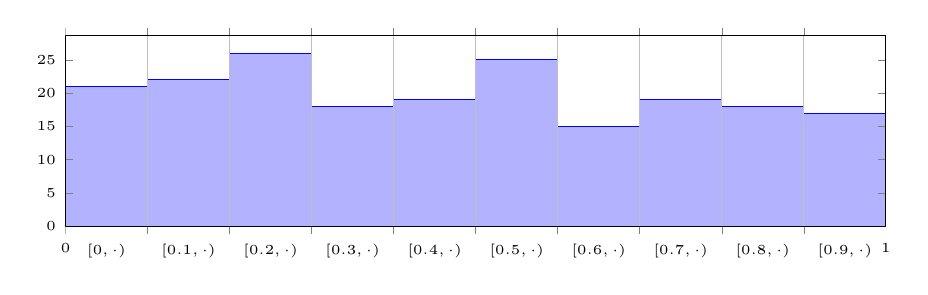
\begin{tikzpicture}
\begin{axis}[
  tiny,
  height=4cm,width=12cm,
  ybar interval,
  ymin=0,
  xmin=0,xmax=1,
  axis on top,
  extra x ticks={0,1},
  extra x tick style={
    grid=none,
    x tick label as interval=false,
    xticklabel=$\pgfmathprintnumber\tick$
  },
  xticklabel={$[\pgfmathprintnumber[fixed]\tick,\cdot)$}
]
	\addplot+[samples=200,hist] {rnd};
\end{axis}
\end{tikzpicture}
\end{codeexample}
	\noindent The example uses the |rnd| method of \pgfname\ which defines |y| to contain uniform random numbers in the range $[0,1]$. Then, it configures |hist|. Note that |hist| has the default |data=y| such that it uses the |y| coordinate as input. Note furthermore that the |x| value is effectively ignored here. The options after |\begin{axis}[...]| are mainly to scale the graphics and to insert the right limits. The |extra x ticks| method is inserted to demonstrate how to add further tick marks without affecting the overall layout. Note that the |extra x tick style| sets |x tick label as interval=false| to disable the special tick handling which is active for the rest of the plot.

	The following keys configure |hist|. If they are provided inside of \meta{options}, the common key prefix |hist/| can be omitted.

	\begin{pgfplotskey}{hist/data=\marg{expression} (initially y)}
		Tells |hist| how to get its data. The common idea is to provide a mathematical \meta{expression} which depends on data supplied by the |\addplot| statement. For example, if you have |\addplot expression|, the \meta{expression} may depend upon |x|, |y| or |z|. In case of an |\addplot table| input routine, the \meta{expression} can employ |\thisrow|\marg{colname} to access the currently active table row in the designated column.
		
		It is also possible to avoid invocations of the math parser. Use \declareandlabel{hist/data value}|=|\marg{value} instead to do so. Here, \meta{value} should be of a numeric constant.

		The initial configuration employs what would usually become the final |y| coordinate as input (to be more precise, the initial value is |data value=\pgfkeysvalueof{/data point/y}|).
	\end{pgfplotskey}

	\begin{pgfplotskeylist}{%
		hist/data min=\marg{min value} (initially /pgfplots/xmin),%
		hist/data max=\marg{max value} (initially /pgfplots/xmax)}%
		Allows to provide the min/max values (the $\underline m$ and $\overline m$) values manually.

		If empty, these v (walues will be deduced from the input data range.
		
		The resulting interval will be splitted into |hist/bins| intervals.

		The initial configuration uses any provided data limits, i.e.\ the (natural) choices |hist/data min=||xmin| and |hist/data max=||xmax|.
	\end{pgfplotskeylist}

	\begin{pgfplotskey}{hist/bins=\marg{number of intervals} (initially 10)}
		Specifies the number of intervals to use.
	\end{pgfplotskey}

	\begin{pgfplotskey}{hist/intervals=\marg{true,false} (initially true)}
		If |intervals=true| (the initial configuration), |hist| will generate $N+1$ coordinates, with
		\[ \underline m = x_0 < x_1 < \dotsb < x_{N} = \overline m \]
		where $[\underline m,\overline m]$ is the data range. In this case, the data points for $x_{N-1}$ and $x_N$ will get the same value, namely the number of elements in the last bin. This is (only) useful in conjunction with |const plot| or |ybar interval|.

		If |intervals=false|, the last data point will be omitted and exactly $N$ coordinates will be generated. In this case, the right end point is not returned explicitly.
	\end{pgfplotskey}

	\begin{pgfplotskey}{hist/cumulative=\marg{true,false} (initially false)}
		Allows to compute a cumulative histogram.

		A cumulative histogram uses the sum of all previous bins and the current one as final value.

		Here is the example from above, this time with |hist/cumulative|:
		
\pgfplotsexpensiveexample
\begin{codeexample}[]
\begin{tikzpicture}
\begin{axis}[
  ybar interval,
  xtick=,% reset from ybar interval
  xticklabel=
    {$[\pgfmathprintnumber\tick,
	   \pgfmathprintnumber\nexttick)$}
]
% a data file containing 8000 normally distributed
% random numbers of mean 0 and variance 1
\addplot+[hist={
		data=x,
		cumulative}]
	file {plotdata/pgfplots.randn.dat};
	
\end{axis}
\end{tikzpicture}
\end{codeexample}
		
	\end{pgfplotskey}

	\begin{pgfplotskey}{hist/density=\marg{true,false} (initially false)}
		\textit{An extension by J\"urnjakob Dugge}
		\vskip\baselineskip
		Enables density estimation mode. If |hist/density| is active, the resulting data points will be renormalized such that the overall ``mass'' equals~$1$. 
\begin{codeexample}[]
\begin{tikzpicture}
\begin{axis}[small,ymin=0,title=\texttt{hist}]
\addplot [
	hist,
	fill=orange!75,
	draw=orange!50!black]
	table [y index=0] {plotdata/pgfplots.randn.dat};
\end{axis}
\end{tikzpicture}
%
\begin{tikzpicture}
\begin{axis}[small,ymin=0, title=\texttt{hist=density}]
\addplot [
	hist=density,
	fill=orange!75,
	draw=orange!50!black]
	table [y index=0] {plotdata/pgfplots.randn.dat};
\end{axis}
\end{tikzpicture}
\end{codeexample}


		The keys |hist/density| and |hist/cumulative| can be combined as well:
\begin{codeexample}[]
\begin{tikzpicture}
\begin{axis}[small,ymin=0, title=\texttt{hist=cumulative}]
\addplot [
	hist=cumulative,
	fill=orange!75,
	draw=orange!50!black]
	table [y index=0] {plotdata/pgfplots.randn.dat};
\end{axis}
\end{tikzpicture}
%
\begin{tikzpicture}
\begin{axis}[small,ymin=0, title=\texttt{hist=\{cumulative,density\}}]
\addplot [
	hist={cumulative,density},
	fill=orange!75,
	draw=orange!50!black]
	table [y index=0] {plotdata/pgfplots.randn.dat};
\end{axis}
\end{tikzpicture}
\end{codeexample}
	\end{pgfplotskey}

	\begin{stylekey}{/pgfplots/hist/handler (initially ybar interval)}
		Allows to change the way the generated coordinates are visualized. The |hist/handler| key is a style, so use |hist/handler/.style={const plot}| to change it.
	\end{stylekey}

	\begin{pgfplotscodekey}{hist/data filter}
		Allows to define coordinate filters, similar to the coordinate filter key |x filter| described in Section~\ref{sec:filters}. The argument |#1| is the coordinate as it has been found after processing |hist/data|. The code is supposed to assign |\pgfmathresult| to contain the result. If |\pgfmathresult| is empty afterwards, it will be skipped. Otherwise, it is supposed to contain a number.

		This filter is applied \emph{before} the histogram is computed. Note that |x filter| and |y filter| are applied \emph{after} the histogram is computed.

		Note that predefined styles like |each nth point| can also be applied to |hist/data| if
		\begin{enumerate}
			\item an asterisk `|*|' is appended to the predefined style's name and
			\item the first argument to the style is |hist/data|.
		\end{enumerate}
		For example, |each nth point*={hist/data}{2}| will skip each second input value of |hist/data| (try it out).
	\end{pgfplotscodekey}

	\begin{pgfplotsxycodekeylist}{
		/pgfplots/hist/data coord trafo,%
		/pgfplots/hist/data coord inv trafo}%
	These keys work in the same way as for |x coord trafo| and |x coord inv trafo|. They are applied to the |hist/data| value before the histogram is evaluated and after the result value is assigned, respectively.

		Note that |hist| will apply the |hist/data coord inv trafo| before it visualizes its results. Consequently, it may be necessary to assign a similar transformation to |x coord trafo| as well.

		See the documentation of |x coord trafo| for more information about custom transformations.
	\end{pgfplotsxycodekeylist}

	\begin{pgfplotskey}{hist/symbolic coords=\marg{list}}
		A style which enables |symbolic x coords| for an axis containing |hist| plots:
\begin{codeexample}[]
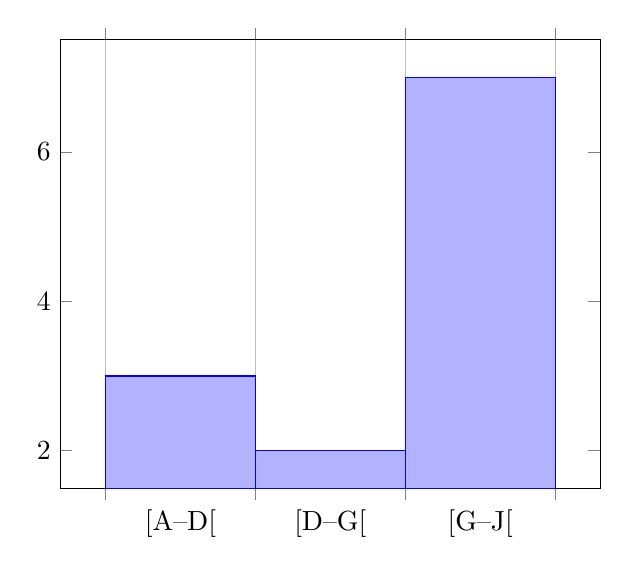
\begin{tikzpicture}
\begin{axis}[
  ybar interval,
  hist/symbolic coords={A,B,C,D,E,F,G,H,I,J},
  xticklabel={[\tick--\nexttick[},
]
    \addplot+[hist={bins=3}]
        table[row sep=\\,y index=0] {
        data\\
		A\\ B\\ A\\ D\\ F\\ J\\
		G\\ J\\ I\\ H\\ I\\ I\\
    };
\end{axis}
\end{tikzpicture}
\end{codeexample}
		The style does two things: first, it defines |hist/data coord trafo| and |hist/data coord inv trafo|, then, it calls |symbolic x coords| with the same argument.

		\paragraph{Attention}: do not use |hist/data=x| or other symbolic values as input when you have |symbolic coords|. Rather than symbolic values, you need to provide \emph{expandable} values like |\pgfkeysvalueof{/data point/x}| (which has the same effect, but directly expands to the correct value).

		Please refer to the documentation of |symbolic x coords| for further details about symbolic coordinates.
	\end{pgfplotskey}
\end{plottype}

\subsubsection{Comb Plots}
Comb plots are very similar to bar plots except that they employ single horizontal/vertical lines instead of rectangles.

\begin{plottype}{xcomb}
\begin{codeexample}[]
\begin{tikzpicture}
\begin{axis}
\addplot+[xcomb] coordinates 
	{(4,0) (1,1) (2,2) 
	 (5,3) (6,4) (1,5)};
\end{axis}
\end{tikzpicture}
\end{codeexample}
\end{plottype}

\begin{plottype}{ycomb}
\begin{codeexample}[]
\begin{tikzpicture}
\begin{axis}
\addplot+[ycomb] plot coordinates
	{(0,3) (1,2) (2,4) (3,1) (4,2)};
\end{axis}
\end{tikzpicture}
\end{codeexample}
\end{plottype}

\subsubsection{Quiver Plots (Arrows)}
\label{sec:pgfplots:quiver2d}
\begin{plottype}[/pgfplots]{quiver=\textcolor{black}{\marg{{\normalfont options with `\texttt{quiver/}' prefix}}}}
	A plot type which draws small arrows, starting at $(x,y)$, in direction of $(u,v)$.
\begin{codeexample}[]
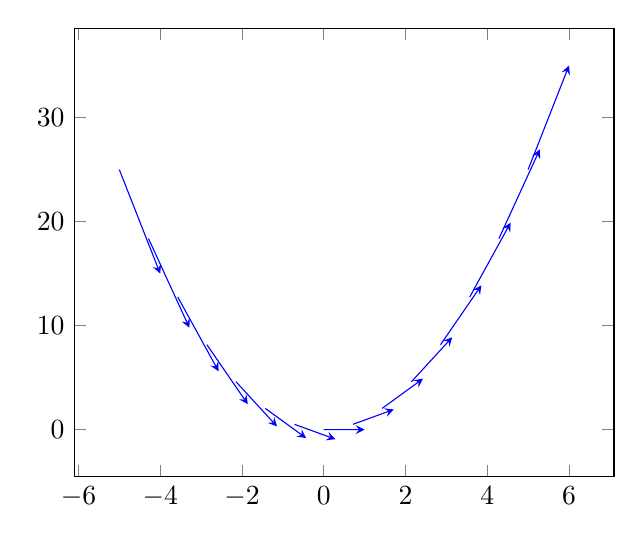
\begin{tikzpicture}
\begin{axis}
	\addplot[blue,
		quiver={u=1,v=2*x},
		-stealth,samples=15] {x^2};
\end{axis}
\end{tikzpicture}
\end{codeexample}

	The base point $(x,y)$ is provided as before; in the example above, it is generated by |plot expression| and yields $(x,x^2)$. The vector direction $(u,v)$ needs to be given in addition. Our example with |quiver/u=1| and |quiver/v=2*x| results in $u=1$ and $v=2x$. Thus, we have defined and visualized a vector field for the derivative of $f(x) = x^2$.

	A common example is to visualize the gradient $(\partial_x f,\partial_y f)(x,y)$ of a two--dimensional function $f(x,y)$:
\pgfplotsexpensiveexample
\begin{codeexample}[]
\begin{tikzpicture}
	\begin{axis}[
		title={$x \exp(-x^2-y^2)$ and its gradient},
		domain=-2:2,
		view={0}{90},
		axis background/.style={fill=white},
	]
		\addplot3[contour gnuplot={number=9,
			labels=false},thick] 
				{exp(0-x^2-y^2)*x};
		\addplot3[blue,
			quiver={
			 u={exp(0-x^2-y^2)*(1-2*x^2)},
			 v={exp(0-x^2-y^2)*(-2*x*y)},
			 scale arrows=0.3,
			},
			-stealth,samples=15]
				{exp(0-x^2-y^2)*x};
	\end{axis}
\end{tikzpicture}
\end{codeexample}
	\noindent The example visualizes $f(x,y) = x\exp(-x^2-y^2)$ using |contour gnuplot| as first step. The options |contour/number| and |contour/labels| provide fine-tuning for the contour and are not of interest here (so is the |axis background| which just improves visibility of contour lines). What we are interested in is the |quiver=| style: it defines |u| and |v| to some two--dimensional expressions. Furthermore, we used |quiver/scale arrows| to reduce the arrow size. The |-stealth| is a \Tikz\ style which configures outgoing arrow styles of type `|stealth|'. The |samples=15| key configures how we get our input data. In our case, we have input data $(x_i,y_j,f(x_i,y_j))$ with $15$ samples for each, $i$ and $j$.

	It is also possible to place quiver plots on a prescribed $z$ value:
\pgfplotsexpensiveexample
\begin{codeexample}[]
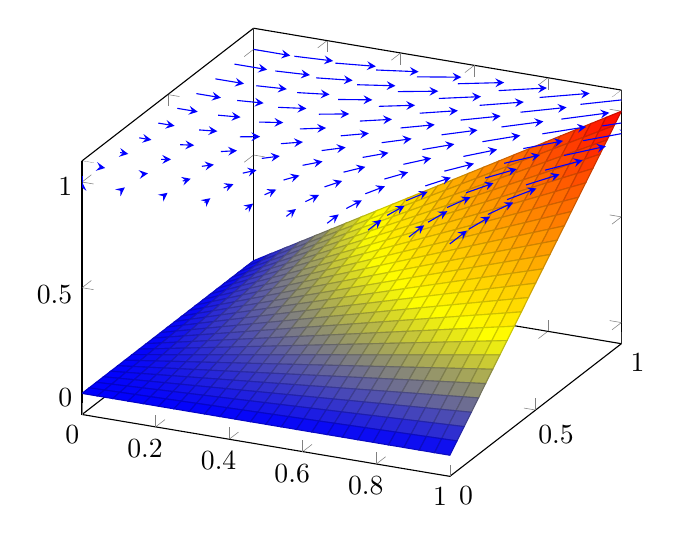
\begin{tikzpicture}
\begin{axis}[
	domain=0:1,
	xmax=1,
	ymax=1,
]
\addplot3[surf] {x*y};
\addplot3[blue,/pgfplots/quiver,
	quiver/u=y,
	quiver/v=x,
	quiver/w=0,
	quiver/scale arrows=0.1,
	-stealth,samples=10] {1};
\end{axis}
\end{tikzpicture}
\end{codeexample}
	\noindent Here, the quiver plots is placed on top of a |surf|. It visualizes the gradient (using a common scale factor of $1/10$ to reduce the arrow lengths). The |quiver/w=0| means that arrows have no $z$ difference, and the |{1}| argument indicates that all start at $(x_i,y_j,1)$. Here, the values $(x_i,y_j)$ are sampled in the |domain=0:1| argument (with |samples=10|), i.e.\ arrows start at $(x_i,y_j,1)$ and end at $(x_i+y_j/10, y_j+x_i/10, 1)$.

	So far, quiver plots do not assume a special sequence of input points. This has two consequences: first, you can plot any vector field by considering just $(x,y) + (u,v)$ (or $(x,y,z) + (u,v,w)$) -- the data doesn't necessarily need to be a two--dimensional function (as opposed to |surf| etc). On the other hand, you need to provide |quiver/scale arrows| manually since |quiver| doesn't know the mesh width in case you provide matrix data\footnote{Actually, I might add something like \texttt{quiver/scale arrows=auto} in the future, I don't know yet. Loops through input data are slow in \TeX, automatic mesh widths computation even more...}.

	Note that quiver plots are currently not available together with logarithmic axes.

	\begin{pgfplotskeylist}{%
		quiver/u=\meta{expression} (initially 0),
		quiver/v=\meta{expression} (initially 0),
		quiver/w=\meta{expression} (initially 0)}
		These keys define how the vector directions $(u,v)$ (or, for three dimensional plots, $(u,v,w)$) shall be set.

		The \meta{expression} can be a constant expression like |quiver/u=1| or |quiver/u=42*5|. It may also depend on the final base point values using the values |x|, |y| or |z| as in the example above. In this context, |x| yields the $x$ coordinate of the point where the vector starts, |y| the $y$ coordinate and so on. 

		\paragraph{Attention:} the fact that |x| refers to \emph{the final $x$ coordinate} means that parametric plots \emph{should use $t$ as variable}\footnote{Sorry for this usability issue.}. Consider the following example:
\begin{codeexample}[]
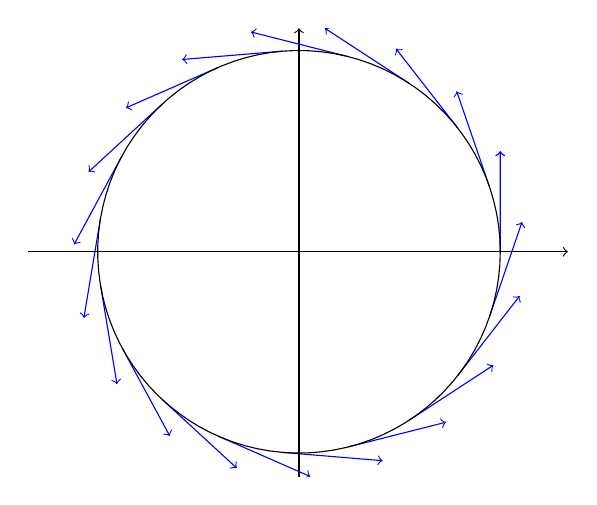
\begin{tikzpicture}
\begin{axis}[axis equal,
 axis lines=middle,
 axis line style={->},
 tick style={color=black},
 xtick=\empty,
 ytick=\empty
]
  \addplot[samples=20, domain=0:2*pi, 
	% the default choice 'variable=\x' leads to 
	% unexpected results here!
	variable=\t,
	quiver={
		u={-sin(deg(t))},
		v={cos(deg(t))},
		scale arrows=0.5},
		->,blue]
	({cos(deg(t))}, {sin(deg(t))});
  \addplot[samples=100, domain=0:2*pi] 
	({cos(deg(x))}, {sin(deg(x))});
\end{axis}
\end{tikzpicture}
\end{codeexample}
	\noindent Here, a parametric plot is used to draw a circle and tangent vectors. The choice |variable=\t| plays a functional role besides naming conventions: it allows to access the parametric variable within the expressions for both |u| and |v|. On the other hand, we could have used |u=y| and |v=-x| since |x| expands to the $x$~coordinate with value |sin(deg(t))| and |y| expands to the $y$~coordinate |cos(deg(t))|.
		
		Another important application is to use \emph{table column references} like |quiver/u=\thisrow{col}| in conjunction with |\addplot table|: 
\begin{codeexample}[]
\begin{tikzpicture}
\begin{axis}[title=Quiver and plot table]
    \addplot[blue,
        quiver={u=\thisrow{u},v=\thisrow{v}},
        -stealth] 
	table 
	{
	x y u v
	0 0 1 0
	1 1 1 1
	2 4 1 4
	3 9 1 6
	4 16 1 8
	};
\end{axis}
\end{tikzpicture}
\end{codeexample}
	\noindent Here, the \meta{expression} employs |\thisrow| which always refers to the actual row of |\addplot table|. 

		Note that \meta{expression} should always be of numeric type (no symbolic input extensions are supported currently).
	\end{pgfplotskeylist}
	\begin{pgfplotskeylist}{%
		quiver/u value=\marg{value} (initially 0),
		quiver/v value=\marg{value} (initially 0),
		quiver/w value=\marg{value} (initially 0)}
		These keys have the \emph{same function} as |quiver/u| and its variants. However, they don't call the math parser, so only single values are allowed (including something like |\thisrow{columnname}|).
	\end{pgfplotskeylist}

	\begin{pgfplotskeylist}{%
		quiver/colored,
		quiver/colored=\marg{color}}
		Allows to define an individual color for each arrow. Omitting the argument `\meta{color}' is identical to |quiver/colored=mapped color| which uses the |point meta| to get colors for every arrow.

		If you just want to set the same color for every arrow, prefer using |\addplot[blue,quiver]| which is more efficient.		
	\end{pgfplotskeylist}

	\begin{pgfplotskey}{quiver/scale arrows=\marg{scale} (initially 1)}
		Allows to rescale the arrows by a factor. This may be necessary if the arrow length is longer than the distance between adjacent base points $(x_i,y_i)$. There may come a feature to rescale them automatically.
	\end{pgfplotskey}

	\begin{pgfplotskey}{quiver/update limits=\mchoice{true,false} (initially true)}
		A boolean indicating whether points $(x,y)  + (u,v)$ shall contribute to the axis limits.		
	\end{pgfplotskey}

	\begin{stylekey}{/pgfplots/quiver/every arrow (initially empty)}
		Allows to provide individual arrow styles.

		The style can contain any \Tikz\ drawing option. It will be evaluated for every individual arrow and may depend upon anything which is available at visualization time. 
		
		In particular, this includes |point meta| data, typically using |\pgfplotspointmetatransformed| $\in [0,1000]$ where~$0$ corresponds to |point meta min| and~$1000$ corresponds to |point meta max|:
\begin{codeexample}[]
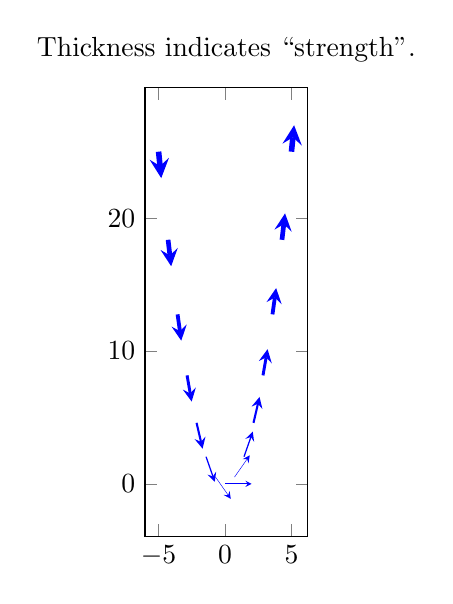
\begin{tikzpicture}
% define some constants:
\def\U{1}
\def\V{2*x}
\def\LEN{(sqrt((\U)^2 + (\V)^2)}

\begin{axis}[axis equal image,
	title=Thickness indicates ``strength''.
]
\addplot[blue,
  point meta={\LEN},
  quiver={
   u={(\U)/\LEN}, v={(\V)/\LEN},
   scale arrows=2,
   every arrow/.append style={
    line width=2pt*\pgfplotspointmetatransformed/1000
   },
  },
  -stealth,samples=15,
] {x^2};
\end{axis}
\end{tikzpicture}
\end{codeexample}
	\noindent In the example, we have some 2d vector field stored in helper constants |\U| and |\V|. The length of each vector is stored in |\LEN| here. The |quiver| plot as such contains unit length vectors -- and the |\LEN| enters an |every arrow| style to get varying |line width|.
		
		An |every arrow| style might also depend upon |mapped color| (provided |point meta| has been set).

		Again, if you do not need individual arrow styles, prefer using a plot style (|cycle list| or argument to |\addplot|) which is more efficient.
	\end{stylekey}

	\begin{pgfplotsxycodekeylist}{%
		quiver/before arrow,%
		quiver/after arrow}%
		Advanced keys for more fine tuning of the display. They allow to install some \TeX\ code manually before or after the drawing operations for single arrows. Both are initially empty.
	\end{pgfplotsxycodekeylist}

	\begin{stylekey}{/pgfplots/quiver/quiver legend}
		A style which redefines |legend image code| in order to produce a suitable legend for |quiver| plots.

		It is implicitly activated whenever |quiver| plot handlers are selected.
\begin{codeexample}[]
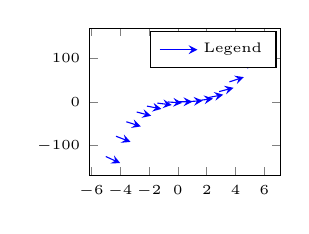
\begin{tikzpicture}
\begin{axis}[tiny]
\addplot[blue, 
	quiver={u=1,v=3*x}, 
	-stealth,
	samples=15] 
	{x^3};
\addlegendentry{Legend}
\end{axis}
\end{tikzpicture}
\end{codeexample}
	\end{stylekey}
\end{plottype}

\subsubsection{Stacked Plots}
\begin{pgfplotskey}{stack plots=\mchoice{x,y,false} (initially false)}
	Allows stacking of plots in either $x$ or $y$ direction. Stacking means to add either $x$- or $y$ coordinates of successive |\addplot| commands on top of each other.
\begin{codeexample}[]
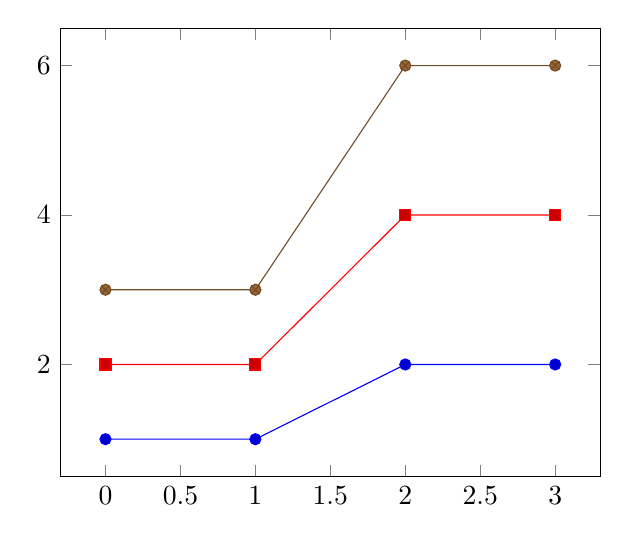
\begin{tikzpicture}
	\begin{axis}[stack plots=y]
	\addplot coordinates
		{(0,1) (1,1) (2,2) (3,2)};
	\addplot coordinates
		{(0,1) (1,1) (2,2) (3,2)};
	\addplot coordinates
		{(0,1) (1,1) (2,2) (3,2)};
	\end{axis}
\end{tikzpicture}
\end{codeexample}

|stack plots| is particularly useful for bar plots. The following examples demonstrate its functionality. Normally, it is advisable to use the styles |ybar stacked| and |xbar stacked| which also set some other options.
\begin{codeexample}[]
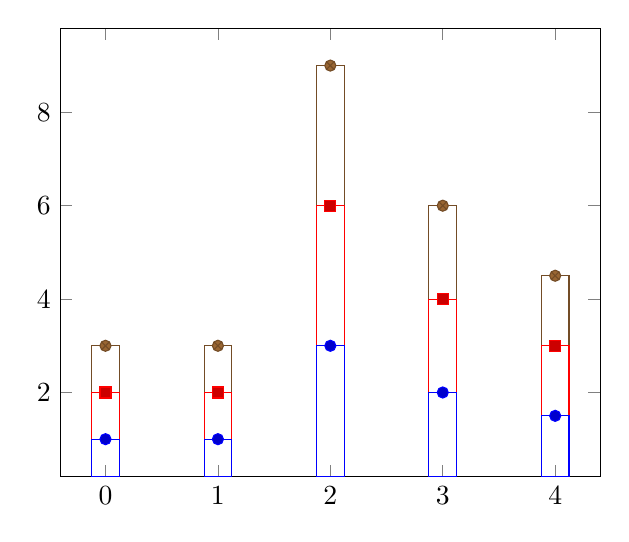
\begin{tikzpicture}
	\begin{axis}[stack plots=y,/tikz/ybar]
	\addplot coordinates
		{(0,1) (1,1) (2,3) (3,2) (4,1.5)};
	\addplot coordinates
		{(0,1) (1,1) (2,3) (3,2) (4,1.5)};
	\addplot coordinates
		{(0,1) (1,1) (2,3) (3,2) (4,1.5)};
	\end{axis}
\end{tikzpicture}
\end{codeexample}

\begin{codeexample}[]
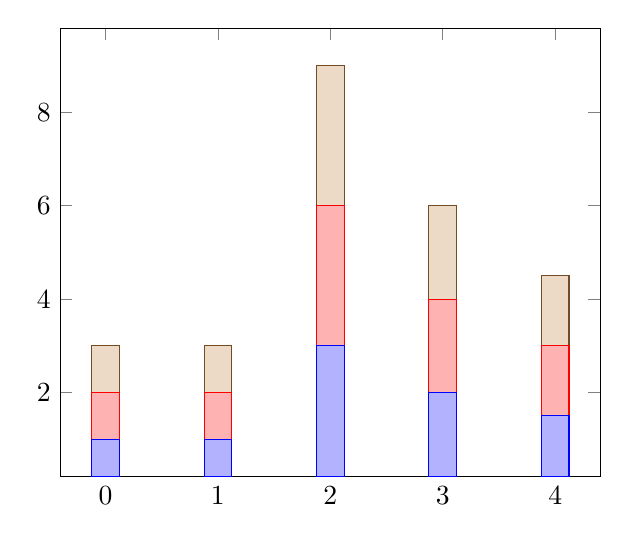
\begin{tikzpicture}
	\begin{axis}[ybar stacked]
	\addplot coordinates
		{(0,1) (1,1) (2,3) (3,2) (4,1.5)};
	\addplot coordinates
		{(0,1) (1,1) (2,3) (3,2) (4,1.5)};
	\addplot coordinates
		{(0,1) (1,1) (2,3) (3,2) (4,1.5)};
	\end{axis}
\end{tikzpicture}
\end{codeexample}

\begin{codeexample}[]
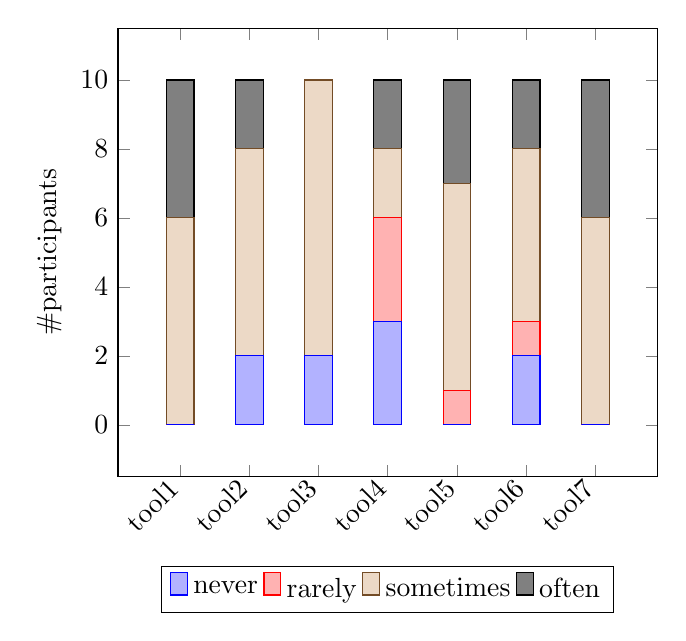
\begin{tikzpicture}
\begin{axis}[
    ybar stacked,
    enlargelimits=0.15,
    legend style={at={(0.5,-0.20)},
      anchor=north,legend columns=-1},
    ylabel={\#participants},
    symbolic x coords={tool1, tool2, tool3, tool4, 
		tool5, tool6, tool7},
    xtick=data,
    x tick label style={rotate=45,anchor=east},
    ]
\addplot+[ybar] plot coordinates {(tool1,0) (tool2,2) 
  (tool3,2) (tool4,3) (tool5,0) (tool6,2) (tool7,0)};
\addplot+[ybar] plot coordinates {(tool1,0) (tool2,0) 
  (tool3,0) (tool4,3) (tool5,1) (tool6,1) (tool7,0)};
\addplot+[ybar] plot coordinates {(tool1,6) (tool2,6)
  (tool3,8) (tool4,2) (tool5,6) (tool6,5) (tool7,6)};
\addplot+[ybar] plot coordinates {(tool1,4) (tool2,2) 
  (tool3,0) (tool4,2) (tool5,3) (tool6,2) (tool7,4)};
\legend{never, rarely, sometimes, often}
\end{axis}
\end{tikzpicture}
\end{codeexample}

\begin{codeexample}[]
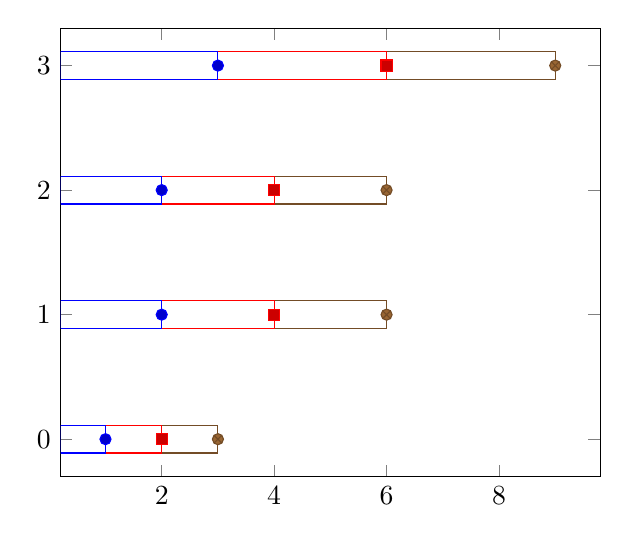
\begin{tikzpicture}
	\begin{axis}[stack plots=x,/tikz/xbar]
	\addplot coordinates
		{(1,0) (2,1) (2,2) (3,3)};
	\addplot coordinates
		{(1,0) (2,1) (2,2) (3,3)};
	\addplot coordinates
		{(1,0) (2,1) (2,2) (3,3)};
	\end{axis}
\end{tikzpicture}
\end{codeexample}
\begin{codeexample}[]

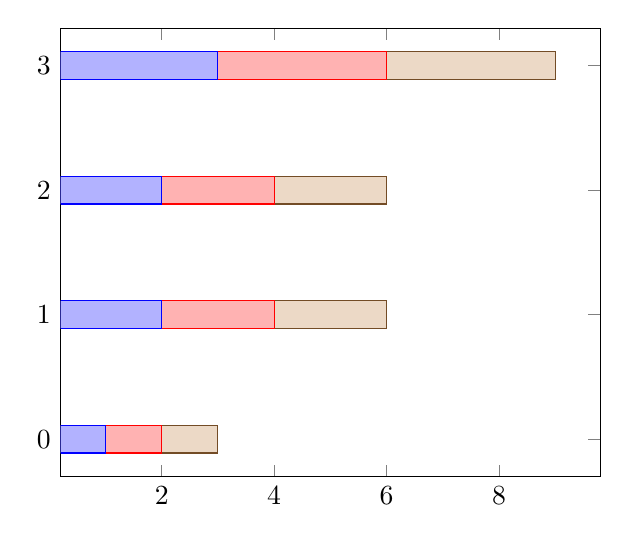
\begin{tikzpicture}
	\begin{axis}[xbar stacked]
	\addplot coordinates
		{(1,0) (2,1) (2,2) (3,3)};
	\addplot coordinates
		{(1,0) (2,1) (2,2) (3,3)};
	\addplot coordinates
		{(1,0) (2,1) (2,2) (3,3)};
	\end{axis}
\end{tikzpicture}
\end{codeexample}
The current implementation for |stack plots| does \emph{not} interpolate missing coordinates. That means stacking will fail if the plots have different grids.
\end{pgfplotskey}

\begin{pgfplotskey}{stack dir=\mchoice{plus,minus} (initially plus)}
	Configures the direction of |stack plots|. The value |plus| will add coordinates of successive plots while |minus| subtracts them.
\end{pgfplotskey}

\begin{pgfplotskey}{reverse stacked plots=\mchoice{true,false} (initially true, default true)}
	Configures the sequence in which stacked plots are drawn. This is more or less a technical detail which should not be changed in any normal case.

	The motivation is as follows: suppose multiple |\addplot| commands are stacked on top of each other and they are processed in the order of appearance. Then, the second plot could easily draw its lines (or fill area) on top of the first one - hiding its marker or line completely. Therefor, \PGFPlots\ reverses the sequence of drawing commands.

	This has the side-effect that any normal \Tikz-paths inside of an axis will also be processed in reverse sequence.
\end{pgfplotskey}

\begin{stylekey}{/pgfplots/xbar stacked=\mchoice{plus,minus} (default plus)}
	A figure-wide style which enables stacked horizontal bars (i.e.\ |xbar| and |stack plots=x|). It also adjusts the legend and tick appearance and assigns a useful |cycle list|.
\end{stylekey}
\begin{stylekey}{/pgfplots/ybar stacked=\mchoice{plus,minus} (default plus)}
	A figure-wide style which enables stacked vertical bars (i.e.\ |ybar| and |stack plots=y|). It also adjusts the legend and tick appearance and assigns a useful |cycle list|.
\end{stylekey}

\begin{stylekey}{/pgfplots/xbar interval stacked=\mchoice{plus,minus} (default plus)}
	A style similar to |/pgfplots/xbar stacked| for the interval based bar plot variant.
\end{stylekey}
\begin{stylekey}{/pgfplots/ybar interval stacked=\mchoice{plus,minus} (default plus)}
	A style similar to |/pgfplots/ybar stacked| for the interval based bar plot variant.
\end{stylekey}

\subsubsection{Area Plots}
Area plots are a combination of |\closedcycle| and |stack plots|. They can be combined with any other plot type.

\begin{codeexample}[]
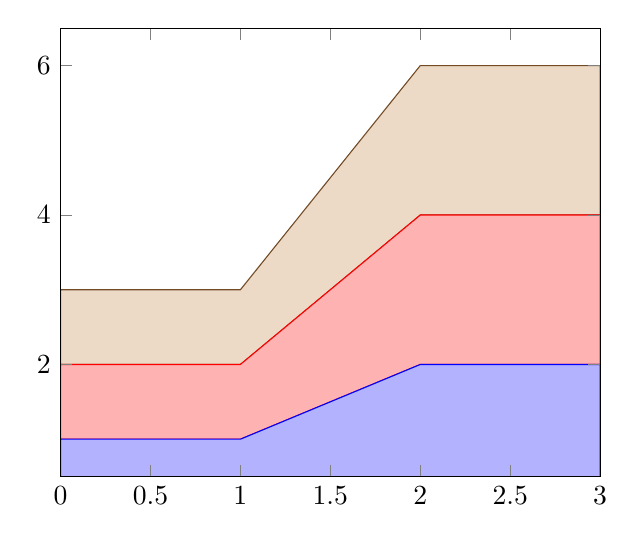
\begin{tikzpicture}
	\begin{axis}[
		stack plots=y,
		area style,
		enlarge x limits=false]
	\addplot coordinates
		{(0,1) (1,1) (2,2) (3,2)} 
		\closedcycle;
	\addplot coordinates
		{(0,1) (1,1) (2,2) (3,2)}
		\closedcycle;
	\addplot coordinates
		{(0,1) (1,1) (2,2) (3,2)}
		\closedcycle;
	\end{axis}
\end{tikzpicture}
\end{codeexample}
\noindent
Area plots may need modified legends, for example using the |area legend| key. Furthermore, one may want to consider the |axis on top| key such that filled areas do not overlap ticks and grid lines. 

\begin{stylekey}{/pgfplots/area style}
	A style which sets
\begin{codeexample}[code only]
\pgfplotsset{
	/pgfplots/area style/.style={%
		area cycle list,
		area legend,
		axis on top,
	}}
\end{codeexample}
\end{stylekey}

\begin{stylekey}{/pgfplots/area cycle list}
	A style which installs a |cycle list| suitable for area plots. The initial configuration of this style simply invokes the |bar cycle list| which does also provide filled plot styles.
\end{stylekey}

\begin{codeexample}[]
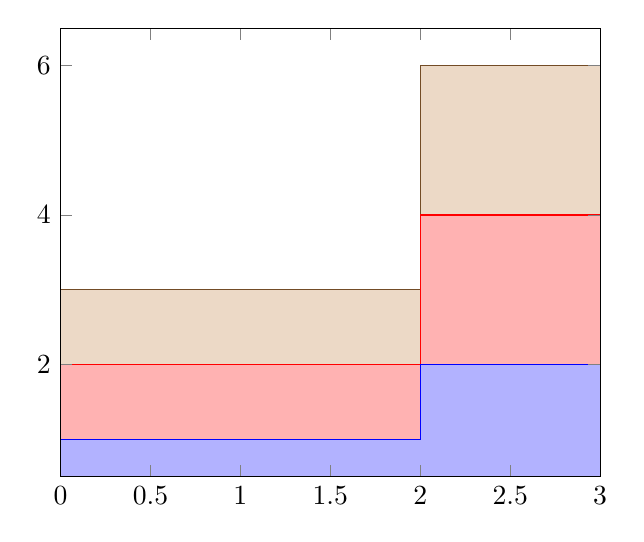
\begin{tikzpicture}
	\begin{axis}[
		const plot,
		stack plots=y,
		area style,
		enlarge x limits=false]
	\addplot coordinates
		{(0,1) (1,1) (2,2) (3,2)} 
		\closedcycle;
	\addplot coordinates
		{(0,1) (1,1) (2,2) (3,2)}
		\closedcycle;
	\addplot coordinates
		{(0,1) (1,1) (2,2) (3,2)}
		\closedcycle;
	\end{axis}
\end{tikzpicture}
\end{codeexample}

\begin{codeexample}[]
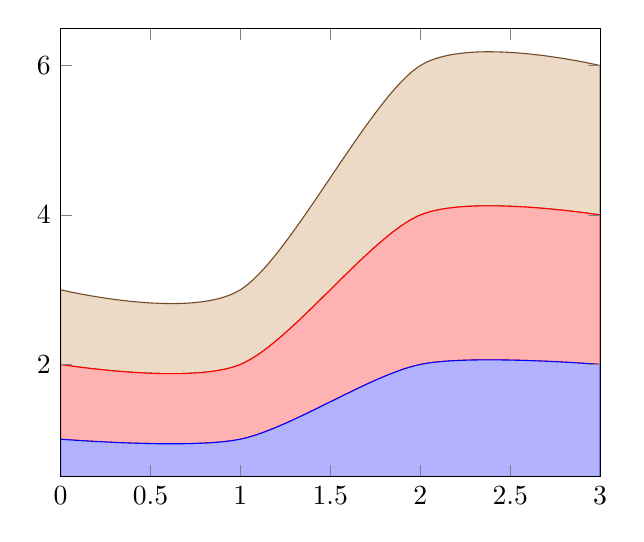
\begin{tikzpicture}
	\begin{axis}[
		smooth,
		stack plots=y,
		area style,
		enlarge x limits=false]
	\addplot coordinates
		{(0,1) (1,1) (2,2) (3,2)} 
		\closedcycle;
	\addplot coordinates
		{(0,1) (1,1) (2,2) (3,2)}
		\closedcycle;
	\addplot coordinates
		{(0,1) (1,1) (2,2) (3,2)}
		\closedcycle;
	\end{axis}
\end{tikzpicture}
\end{codeexample}

\begin{codeexample}[]
\pgfplotstableread{pgfplots.timeseries.dat}\loadedtable
\pgfplotstabletypeset\loadedtable
\end{codeexample}
\begin{codeexample}[]
\pgfplotstableread
	{pgfplots.timeseries.dat}
	{\loadedtable}

\begin{tikzpicture}
	\begin{axis}[
		ymin=0,
		minor tick num=4,
		enlarge x limits=false,
		axis on top,
		every axis plot post/.append style=
			{mark=none},
		const plot,
		legend style={
			area legend,
			at={(0.5,-0.15)},
			anchor=north,
			legend columns=-1}]

	\addplot[draw=blue,fill=blue!30!white]
	 table[x=time,y=1minload] from \loadedtable
		\closedcycle;
	\addplot table[x=time,y=nodes] from \loadedtable;
	\addplot table[x=time,y=cpus] from \loadedtable;
	\addplot table[x=time,y=processes] 
		from \loadedtable;
	\legend{1min load,nodes,cpus,processes}
	\end{axis}
\end{tikzpicture}
\end{codeexample}

\begin{codeexample}[width=4cm]
\pgfplotstableread{pgfplots.timeseries.dat}\loadedtable

\begin{tikzpicture}
	\begin{axis}[
		ymin=0,
		minor tick num=4,
		enlarge x limits=false,
		const plot,
		axis on top,
		stack plots=y,
		cycle list={%
			{blue!70!black,fill=blue},%
			{blue!60!white,fill=blue!30!white},%
			{draw=none,fill={rgb:red,138;green,82;blue,232}},%
			{red,thick}%
		},
		ylabel={Mem [GB]},
		legend style={
			area legend,
			at={(0.5,-0.15)},
			anchor=north,
			legend columns=2}]

	\addplot table[x=time,y=memused]      from \loadedtable \closedcycle;
	\addplot table[x=time,y=memcached]    from \loadedtable \closedcycle;
	\addplot table[x=time,y=membuf]       from \loadedtable \closedcycle;
	\addplot+[stack plots=false]
			 table[x=time,y=memtotal]     from \loadedtable;
	\legend{Memory used,Memory cached,Memory buffered,Total memory}
	\end{axis}
\end{tikzpicture}
\end{codeexample}

\subsubsection{Scatter Plots}
\label{sec:pgfplots:scatter:2d}
The most simple scatter plots produce the same as the line plots above -- but they contain only markers. They are enabled using the |only marks| key of \Tikz.
\begin{plottype}{only marks}
Draws a simple scatter plot: all markers have the same appearance.
\begin{codeexample}[]
\begin{tikzpicture}
	\begin{axis}[enlargelimits=false]
	\addplot+[only marks,samples=400]
		{rand};
	\end{axis}
\end{tikzpicture}
\end{codeexample}
	The |only marks| visualization style simply draws marks at every coordinate. Marks can be set with |mark=|\meta{mark name} and marker options like size and color can be specified using the |mark options=|\meta{style options} key (or by modifying the |every mark| style). The available markers along with the accepted style options can be found in Section~\ref{sec:markers} on page~\pageref{sec:markers}.
\end{plottype}

\label{pgfplots:scatter}
More sophisticated scatter plots change the marker appearance for each data point. An example is that marker colors depend on the magnitude of function values $f(x)$ or other provided coordinates. The term ``scatter plot'' will be used for this type of plot in the following sections.

Scatter plots require ``source'' coordinates. These source coordinates can be the $y$ coordinate, or explicitly provided additional values.

\begin{plottype}[/pgfplots]{scatter}
	Enables marker appearance modifications. The default implementation acquires ``source coordinates'' for every data point (see |scatter src| below) and maps them linearly into the current color map. The resulting color is used as draw and fill color of the marker.

\begin{codeexample}[]
\begin{tikzpicture}
	\begin{axis}
	\addplot+[scatter,only marks,
		 samples=50,scatter src=y]
		{x-x^2};
	\end{axis}
\end{tikzpicture}
\end{codeexample}

	The key |scatter| is simply a boolean variable which enables marker modifications. It applies only to markers and it can be combined with any other plot type.

\begin{codeexample}[]
\begin{tikzpicture}
	\begin{axis}
	\addplot+[scatter,
		 samples=50,scatter src=y]
		{x^3};
	\end{axis}
\end{tikzpicture}
\end{codeexample}
\end{plottype}

Scatter plots can be configured using a set of options. One of them is mandatory, the rest allows fine grained control over marker appearance options.

\begin{pgfplotskey}{scatter src=\mchoice{none,\meta{expression},x,y,z,f(x),explicit,explicit symbolic} (initially none)}
\label{pgfplots:scatter:src}
	This key is necessary for any scatter plot and it is set to |f(x)| as soon as |scatter| is activated and no different choice has been made. It needs to be provided as \meta{option} for |\addplot| to configure the value used to determine marker appearances. Actually, |scatter src| is nothing but an alias for |point meta|, so the main documentation for this key is on page~\pageref{pgfplots:pointmeta}. However, we summarize the choices here together with scatter plot examples.

	Usually, |scatter src| provides input data (numeric or string type) which is used to determine colors and other style options for markers.
	The default configuration expects numerical data which is mapped linearly into the current color map.

	The value of |scatter src| determines how to get this data: the choices \declaretext{x}, \declaretext{y} and \declaretext{z} will use either the $x$, $y$ or $z$ coordinates to determine marker options. Any coordinate filters, logarithms or stacked-plot computations have already been applied to these values (use |rawx|, |rawy| and |rawz| for unprocessed values). The special choice |f(x)| is the same as |y| for two dimensional plots and the same as |z| for three dimensional plots. The choice \declaretext{explicit} expects the scatter source data as additional coordinate from the coordinate input streams (see Section~\ref{pgfplots:providing:input} for how to provide input meta data or below for some small examples). They will be treated as numerical data. The choice \declaretext{explicit symbolic} also expects scatter source data as additional meta information for each input coordinate, but it treats them as strings,  not as numerical data. Consequently, no arithmetics is performed. It is the task of the scatter plot style to do something with it. See, for example, the |scatter/classes| style below.
	Finally, it is possible to provide an arbitrary mathematical expression which involves zero, one or more of the values \declaretext{x} (the current $x$ coordinate), \declaretext{y} (the current $y$ coordinate) or \declaretext{z} (the current $z$ coordinate, if any).

	If data is read from tables, mathematical expressions might also involve |\thisrow|\marg{column name} or |\thisrowno|\marg{column index} to access any of the table cells in the current row.

	Here are examples for how to provide data for the choices \declaretext{explicit} and \declaretext{explicit symbolic}.
\begin{codeexample}[code only]
\begin{tikzpicture}
	\begin{axis}
		% provide color data explicitly using [<data>]
		% behind coordinates:
		\addplot+[scatter,scatter src=explicit]
			coordinates {
				(0,0) [1.0e10]
				(1,2) [1.1e10]
				(2,3) [1.2e10]
				(3,4) [1.3e10]
				% ...
			};

        % Assumes a datafile.dat like
        % xcolname  ycolname    colordata
        % 0         0           0.001
        % 1         2           0.3
        % 2         2.1         0.4
        % 3         3           0.5
        % ...
        % the file may have more columns.
		\addplot+[scatter,scatter src=explicit]
			table[x=xcolname,y=ycolname,meta=colordata] 
				{datafile.dat};
		% Same data as last example: 
		\addplot+[scatter,scatter src=\thisrow{colordata}+\thisrow{ycolname}]
			table[x=xcolname,y=ycolname] 
				{datafile.dat};

        % Assumes a datafile.dat like
        % 0         0           0.001
        % 1         2           0.3
        % 2         2.1         0.4
        % 3         3           0.5
        % ...
        % the first three columns will be used here:
		\addplot+[scatter,scatter src=explicit]
			file {datafile.dat};
	\end{axis}
\end{tikzpicture}
\end{codeexample}

	Please note that |scatter src|$\neq$|none| results in computational work even if |scatter=false|.
\end{pgfplotskey}

\begin{stylekey}{/pgfplots/scatter/use mapped color=\marg{options for each marker} (initially draw=mapped color!80!black,fill=mapped color)}
	This style is installed by default. When active, it recomputes the color |mapped color| for every processed point coordinate by transforming the |scatter src| coordinates into the current color map linearly. Then, it evaluates the options provided as \meta{options for each marker} which are expected to depend on |mapped color|.

	The user interface for color maps is described in Section~\ref{pgfplots:colormap}.
\begin{codeexample}[]
\begin{tikzpicture}
\begin{axis}[title=Default arguments]
\addplot+[scatter,scatter src=y]
	{2*x+3};
\end{axis}
\end{tikzpicture}
\end{codeexample}

\begin{codeexample}[]
\begin{tikzpicture}
\begin{axis}[
	title=Black fill color and varying draw color,
	scatter/use mapped color=
		{draw=mapped color,fill=black}]
\addplot+[scatter,scatter src=y]
	{2*x+3};
\end{axis}
\end{tikzpicture}
\end{codeexample}

\begin{codeexample}[]
\begin{tikzpicture}
\begin{axis}[
	title=Black draw color and varying fill color,
	scatter/use mapped color=
		{draw=black,fill=mapped color}]
\addplot+[scatter,scatter src=y]
	{2*x+3};
\end{axis}
\end{tikzpicture}
\end{codeexample}
	This key is actually a style which redefines |@pre marker code| and |@post marker code| (see below).

	\paragraph{Remark:} The style |use mapped color| \emph{re}defines |@pre marker code| and |@post marker code|. There is a starred variant \declareandlabel{use mapped color*} which \emph{appends} the functionality while keeping the old marker code.
\end{stylekey}

\begin{stylekey}{/pgfplots/scatter/classes=\marg{styles for each class name}}
\label{pgfplots:scatterclasses}
	A scatter plot style which visualizes points using several classes. The style assumes that every point coordinate has a class label attached, that means the choice |scatter src=explicit symbolic| is assumed\footnote{If \texttt{scatter src} is not \texttt{explicit symbolic}, we expect a numeric argument which is rounded to the nearest integer. The resulting integer is used a class label. If that fails, the numeric argument is truncated to the nearest integer. If that fails as well, the point has no label.}. A class label can be a number, but it can also be a symbolic constant. Given class labels for every point, \meta{styles for each class name} contains a comma-separated list which associates appearance options to each class label.

\begin{codeexample}[]
\begin{tikzpicture}
\begin{axis}[scatter/classes={
	a={mark=square*,blue},%
	b={mark=triangle*,red},%
	c={mark=o,draw=black}}]

	% \addplot[] is better than \addplot+[] here:
	% it avoids scalings of the cycle list
	\addplot[scatter,only marks,
		scatter src=explicit symbolic]
		coordinates {
			(0.1,0.15)  [a]
			(0.45,0.27) [c]
			(0.02,0.17) [a]
			(0.06,0.1)  [a]
			(0.9,0.5)   [b]
			(0.5,0.3)   [c]
			(0.85,0.52) [b]
			(0.12,0.05) [a]
			(0.73,0.45) [b]
			(0.53,0.25) [c]
			(0.76,0.5)  [b]
			(0.55,0.32) [c]
		};
\end{axis}
\end{tikzpicture}
\end{codeexample}
In this example, the coordinate |(0.1,0.15)| has the associated label `|a|' while |(0.45,0.27)| has the label `|c|' (see Section~\ref{sec:addplot} for details about specifying point meta data). Now, the argument to |scatter/classes| contains styles for every label -- for label `|a|', square markers will be drawn in color blue. 

The generation of a legend works as for a normal plot -- but |scatter/classes| requires one legend entry for every provided class. It communicates the class labels to the legend automatically. It works as if there had been different |\addplot| commands, one for every class label.

It is also possible to provide |scatter/classes| as argument to a single plot, allowing different scatter plots in one axis.
\begin{codeexample}[]
\begin{tikzpicture}
\begin{axis}[legend pos=south east]
	% The data file contains:
	% x     y      label
	% 0.1   0.15   a 
	% 0.45  0.27   c 
	% 0.02  0.17   a 
	% 0.06  0.1    a 
	% 0.9   0.5    b 
	% 0.5   0.3    c 
	% 0.85  0.52   b 
	% 0.12  0.05   a 
	% 0.73  0.45   b 
	% 0.53  0.25   c 
	% 0.76  0.5    b 
	% 0.55  0.32   c 
    \addplot[
		% clickable coords={\thisrow{label}}, 
		scatter/classes={
			a={mark=square*,blue},%
			b={mark=triangle*,red},%
			c={mark=o,draw=black,fill=black}%
		},
		scatter,only marks,
		scatter src=explicit symbolic]
	table[x=x,y=y,meta=label]
			{plotdata/scattercl.dat};

	\addplot coordinates 
		{(0.1,0.1) (0.5,0.3) (0.85,0.5)};
	\legend{Class 1,Class 2,Class 3,Line}
\end{axis}
\end{tikzpicture}
\end{codeexample}

In general, the format of \meta{styles for each class name} is a comma separated list of \meta{label}|=|\marg{style options}.

\paragraph{Attention:} The keys |every mark| and |mark options| have \emph{no effect} when used inside of \meta{styles for each class name}! So, instead of assigning |mark options|, you can simply provide the options directly. They apply only to markers anyway.

\paragraph{Remark:} To use |\label| and |\ref| in conjunction with |scatter/classes|, you can provide the class labels as optional arguments to |\label| in square brackets:

\begin{codeexample}[code only]
\addplot[
	scatter/classes={
		a={mark=square*,blue},%
		b={mark=triangle*,red},%
		c={mark=o,draw=black,fill=black}%
	},
	scatter,only marks,
	scatter src=explicit symbolic]
	% [and coordinate input here... ]
	;

\label[a]{label:for:first:class}
\label[b]{label:for:second:class}
\label[c]{label:for:third:class}

...
First class is \ref{label:for:first:class}, second is \ref{label:for:second:class}.
\end{codeexample}

\paragraph{Remark:} It is possible to click into the plot to display labels with mouse popups, see the |clickable coords| key of the |clickable| library.

	\paragraph{Remark:} The style |scatter/classes| \emph{re}defines |@pre marker code| and |@post marker code|. There is a starred variant \declareandlabel{scatter/classes*} which \emph{appends} the functionality while keeping the old marker code.
\end{stylekey}

\begin{pgfplotskeylist}{%
	nodes near coords=\marg{content} (default \textbackslash pgfmathprintnumber\textbackslash pgfplotspointmeta),
	nodes near coords*=\marg{content} (default \textbackslash pgfmathprintnumber\textbackslash pgfplotspointmeta)}
	A |scatter| plot style which places text nodes near every coordinate.

\begin{codeexample}[]
\begin{tikzpicture}
\begin{axis}[nodes near coords]
	\addplot+[only marks] coordinates {
		(0.5,0.2) (0.2,0.1) (0.7,0.6) 
		(0.35,0.4) (0.65,0.1)};
\end{axis}
\end{tikzpicture}
\end{codeexample}
	The \meta{content} is, if nothing else has been specified, the content of the ``point meta'', displayed using the default \meta{content}=|\pgfmathprintnumber{\pgfplotspointmeta}|. The macro |\pgfplotspointmeta| contains whatever has been selected by the |point meta| key, it defaults to the $y$ coordinate for two dimensional plots and the $z$ coordinate for three dimensional plots.

	Since |point meta=explicit symbolic| allows to treat string data, you can provide textual descriptions which will be shown inside of the generated nodes\footnote{In this case, the |\textbackslash pgfmathprintnumber| will be skipped automatically.}:

\begin{codeexample}[]
\begin{tikzpicture}
\begin{axis}[nodes near coords,enlargelimits=0.2]
	\addplot+[only marks,
		point meta=explicit symbolic] 
	coordinates {
		(0.5,0.2) [(1)]
		(0.2,0.1) [(2)]
		(0.7,0.6) [(3)]
		(0.35,0.4) [(4)]
		(0.65,0.1) [(5)]
	};
\end{axis}
\end{tikzpicture}
\end{codeexample}
	The square brackets are the way to provide explicit |point meta| for |plot coordinates|. Please refer to the documentation of |plot file| and |plot table| for how to get point meta from files.

	The \meta{content} can also depend on something different than |\pgfplotspointmeta|. But since \meta{content} is evaluated during |\end{axis}|, \PGFPlots\ might not be aware of any special information inside of \meta{content} -- you'll need to communicate it to \PGFPlots\ with the |visualization depends on| key as follows:
\begin{codeexample}[width=3cm]
\begin{tikzpicture}
	\begin{axis}[enlargelimits=0.2]
		\addplot[
		  scatter,mark=*,only marks,
		  % we use 'point meta' as color data...
		  point meta=\thisrow{color},
		  % ... therefore, we can't use it as argument for nodes near coords ...
		  nodes near coords*={$(\pgfmathprintnumber[frac]\myvalue)$},
		  % ... which requires to define a visualization dependency:
		  visualization depends on={\thisrow{myvalue} \as \myvalue},
		] 
		table {
			x      y    color   myvalue
			0.5    0.2  1       0.25   
			0.2    0.1  2       1.5    
			0.7    0.6  3       0.75   
			0.35   0.4  4       0.125  
			0.65   0.1  5       2      
		};
	\end{axis}
\end{tikzpicture}
\end{codeexample}
	\noindent The example uses a |scatter| plot to get different colors, where the |scatter src| (or, equivalently, |point meta|) is already used to define the markers color. In addition to the colored |scatter| plot, we'd like to add |nodes near coords|, where the displayed nodes should contain |\thisrow{myvalue}|. To do so, we define |scatter,point meta=\thisrow{color}| (just as described in the previous sections). Furthermore, we use \declare{nodes near coords*} in order to \emph{combine} different |scatter| styles (see below for details). The value for |nodes near coords*| depends on |\thisrow{myvalue}|, but we can't use |\pgfplotspointmeta| (which is already occupied). Thus, we communicate the additional input data by means of |visualization depends on={\thisrow{myvalue} \as \myvalue}|. The statement defines a new macro, |\myvalue|, and assigns the value |\thisrow{myvalue}|. Furthermore, it configures \PGFPlots\ to remember this particular macro and its contents until |\end{axis}| (see the documentation for |visualization depends on| for details).
	

	The style |nodes near coords| might be useful for bar plots, see |ybar| for an example of |nodes near coords|.

	\paragraph{Remarks and Details:}
	\begin{itemize}
		\item |nodes near coords| uses the same options for line styles and colors as the current plot. This may be changed using the style |every node near coord|, see below.

		\item |nodes near coords| is actually one of the |scatter| plot styles. It redefines |scatter/@pre marker code| to generate several \Tikz\ |\node| commands.

		In order to use |nodes near coords| together with other |scatter| plot styles (like |scatter/use mapped color| or |scatter/classes|), you may append a star to each of these keys. The variant \declareandlabel{nodes near coords*} will \emph{append} code to |scatter/@pre marker code| without overwriting the previous value.
		\item Consider using |enlargelimits| together with |nodes near coords| if text is clipped away.
		\item Currently |nodes near coords| does not work satisfactorily for |ybar interval| or |xbar interval|, sorry.

	\end{itemize}
\end{pgfplotskeylist}

\begin{stylekey}{/pgfplots/every node near coord}
	A style used for every node generated by |nodes near coords|. It is initially empty.
\end{stylekey}

\begin{pgfplotskey}{nodes near coords align=\marg{alignment method} (initially auto)}
	Specifies how to align nodes generated by |nodes near coords|. 

	Possible choices for \meta{alignment method} are

	\begin{description}
		\item[]\declare{auto} uses |horizontal| if the $x$ coordinates are shown or |vertical| in all other cases. This checks the current value of |point meta|.
		\item[]\declare{horizontal} uses |left| if |\pgfplotspointmeta| $<0$ and |right| otherwise.
		\item[]\declare{vertical}   uses |below| if |\pgfplotspointmeta| $<0$ and |above| otherwise.
		\item[] It is also possible to provide any \Tikz\ alignment option such as |anchor=north east|, |below| or something like that. It is also allowed to provide multiple options.
	\end{description}
\end{pgfplotskey}


\begin{pgfplotsxycodekeylist}{
	scatter/@pre marker code,
	scatter/@post marker code}
	These two keys constitute the public interface which determines the marker appearance depending on scatter source coordinates.

	Redefining them allows fine grained control even over marker types, line styles and colors.

	The scatter plot algorithm works as follows:
\begin{enumerate} 
\item The scatter source coordinates form a data stream whose data limits are computed additionally to the axis limits. This step is skipped for |symbolic| meta data.
\item Before any markers are drawn, a linear coordinate transformation from these data limits to the interval $[0.0,1000.0]$ is initialised. 
\item Every scatter source coordinate\footnote{During the evaluation, the public macros \texttt{\textbackslash pgfplotspointmeta} and \texttt{\textbackslash pgfplotspointmetarange} indicate the source coordinate and the source coordinate range in the format $a:b$ (for log--axis, they are given in fixed-point representation and for linear axes in floating point).} will be transformed linearly and the result is available as macro |\pgfplotspointmetatransformed| $ \in [0.0,1000.0]$.

The decision is thus based on per thousands of the data range. The transformation is skipped for |symbolic| meta data (and the meta data is simply contained in the mentioned macro).
\item The \pgfname\ coordinate system is translated such that |(0pt,0pt)| is the plot coordinate.
\item The code of |scatter/@pre marker code| is evaluated (without arguments).
\item The standard code which draws markers is evaluated.
\item The code of |scatter/@post marker code| is evaluated (without arguments).
\end{enumerate}
	The idea is to generate a set of appearance keys which depends on |\pgfplotspointmetatransformed|. Then, a call to |\scope|\oarg{generated keys} as |@pre| code and the associated |\endscope| as |@post| code will draw markers individually using \oarg{generated keys}.

A technical example is shown below. It demonstrates how to write user defined routines, in this case a three--class system\footnote{Please note that you don't need to copy this particular example: the multiple--class example is also available as predefined style \texttt{scatter/classes}.}.
\begin{codeexample}[]
\begin{tikzpicture}
% Low-Level scatter plot interface Example: 
% use three different marker classes 
% 0% - 30%   : first class
% 30% - 60%  : second class
% 60% - 100% : third class
\begin{axis}[
scatter/@pre marker code/.code={%
   \ifdim\pgfplotspointmetatransformed pt<300pt
      \def\markopts{mark=square*,fill=blue}%
   \else
      \ifdim\pgfplotspointmetatransformed pt<600pt
         \def\markopts{mark=triangle*,fill=orange}%
      \else
         \def\markopts{mark=pentagon*,fill=red}%
      \fi
   \fi
   \expandafter\scope\expandafter[\markopts]
},%
scatter/@post marker code/.code={%
   \endscope
}]

\addplot+[scatter,scatter src=y,
	samples=40]
   {sin(deg(x))};
   
\end{axis}
\end{tikzpicture}
\end{codeexample}
Please note that |\ifdim| compares \TeX\ lengths, so the example employs the suffix |pt| for any number used in this context. That doesn't change the semantics. The two (!) |\expandafter| constructions make sure that |\scope| is invoked with the \emph{content} of |\markopts| instead of the macro name |\markopts|.
\end{pgfplotsxycodekeylist}

\subsubsection{1D Colored Mesh Plots}
\label{sec:1d:mesh}
\begin{plottype}[/pgfplots]{mesh}
	Uses the current color map to determine colors for each fixed line segment. Each line segment will get the same color.
\begin{codeexample}[]
\begin{tikzpicture}
	\begin{axis}
	\addplot[mesh] {x+sin(deg(x))};
	\end{axis}
\end{tikzpicture}
\end{codeexample}
	The color data is per default the $y$ value of the plot. It can be reconfigured using the |point meta| key (which is actually the same as |scatter src|). The following example provides the color data explicitly for |plot coordinates|, using the square bracket notation.
\begin{codeexample}[]
\begin{tikzpicture}
	\begin{axis}
	\addplot[mesh,point meta=explicit] 
		coordinates {
			(0,0)   [0]
			(1,0.1) [1]
			(2,0.1) [2]
			(3,0.3) [3]
			(4,0.3) [4]
		};
	\end{axis}
\end{tikzpicture}
\end{codeexample}
	This one-dimensional |mesh| plot is actually a special case of the twodimensional mesh plots, so more detailed configuration, including how to change the color data, can be found in Section~\ref{sec:2d:mesh}.

\end{plottype}


\subsubsection{Interrupted Plots}
\index{Interrupted Plots}%
\label{pgfplots:interrupt}%
Sometimes it is desirable to draw parts of a single plot separately, without connection between the parts (discontinuities). \PGFPlots\ offers two ways to generate interrupted plots: either using |empty line|s or by providing |unbounded coords|.

The first way is simple; it needs no extra key (only |\pgfplotsset{compat=1.4}| or newer in your preamble):
\begin{codeexample}[]
\begin{tikzpicture}
\begin{axis}[
	title=Interrupted data plot]

	\addplot coordinates {
		(0,0) (10,50) (20,100) (30,200) 

		(50,600) (60,800) (80,1000)
	};
\end{axis}
\end{tikzpicture}
\end{codeexample}
\noindent Here, \PGFPlots\ runs with the default configuration |empty line=auto| which interpretes empty lines as ``jump'' markers. This works for any data input method, i.e.\ using |\addplot coordinates|, |\addplot table|, and |\addplot file|.


The second way to generate interrupted plots addresses the case where |empty line|s are unavailable or impossible (due to limitations of the tool generating the data file, for example). In this case, interrupted plots can be achieved using the |unbounded coords| key combined with coordinate values |nan|, |inf| or |-inf|.

\begin{pgfplotskey}{unbounded coords=\mchoice{discard,jump} (initially discard)}
	This key configures what to do if one or more coordinates of a single point are unbounded. Here, unbounded means it is either $\pm \infty$ (|+inf| or |-inf|) or it has the special ``not--a--number'' value |nan|.

	The initial setting \declaretext{discard} discards the complete point and a warning is issued in the log file\footnote{The warning can be disabled with \texttt{filter discard warning=false}.}. This setting has the same effect as if the unbounded point did not occur: \PGFPlots\ will interpolate between the bounded adjacent points.

	The alternative \declaretext{jump} allows interrupted plots: it provides extra checking for these coordinates and does not interpolate over them; only those line segments which are adjacent to unbounded coordinates will be skipped. 
\begin{codeexample}[]
\begin{tikzpicture}
\begin{axis}[
	title=Discarding unbounded coords,
	unbounded coords=discard]

	\addplot coordinates {
		(0,0) (10,50) (20,100) (30,200) 
		(40,inf) (50,600) (60,800) (80,1000)
	};
\end{axis}
\end{tikzpicture}
\begin{tikzpicture}
\begin{axis}[
	title=Jumps at unbounded coords,
	unbounded coords=jump]
	\addplot coordinates {
		(0,0) (10,50) (20,100) (30,200) 
		(40,inf) (50,600) (60,800) (80,1000)
	};
\end{axis}
\end{tikzpicture}
\end{codeexample}

	For plot expression and its friends, it is more likely to get very large floating point numbers instead of |inf|. In this case, consider using the |restrict x to domain| key described on page~\pageref{key:restrict:x:to:domain}.

	The |unbounded coords=jump| method does also work for mesh/surface plots: every face adjacent to an unbounded coordinate will be discarded in this case. The following example sets up a (cryptic) coordinate filter which cuts out a quarter of the domain and replaces its values with |nan|:

\pgfplotsexpensiveexample
\begin{codeexample}[]
\begin{tikzpicture}
\begin{axis}[
  unbounded coords=jump,
  % A technical filter to cut out 
  % the x<0 and y<0 edge.
  filter point/.code={%
    \pgfmathparse
      {\pgfkeysvalueof{/data point/x}<0}%
    \ifpgfmathfloatcomparison
      \pgfmathparse
        {\pgfkeysvalueof{/data point/y}<0}%
      \ifpgfmathfloatcomparison
        \pgfkeyssetvalue{/data point/x}{nan}%
      \fi
    \fi
  },
  ]
  \addplot3[surf] {exp(-sqrt(x^2 + y^2))};
\end{axis}
\end{tikzpicture}
\end{codeexample}
\end{pgfplotskey}

More about this coordinate filtering can be found in Section~\ref{sec:filters} ``Skipping Or Changing Coordinates -- Filters''.

\subsubsection{Patch Plots}
Patch Plots visualize a sequence of one or more triangles (or other sorts of patches). These triangles can be drawn with a single color (|shader=flat| and |shader=faceted interp|) or with interpolated colors (|shader=interp|).

There are both two- and three-dimensional patch plots, both with the same interface and the same keys. Therefore, the reference documentation for patch plots can be found in Section~\ref{sec:pgfplots:3d:patch} together with three--dimensional patch plots.

\label{sec:pgfplots:2d:patch}
}
